\documentclass[%
11pt,%
%oneside,%
twoside,%
%twocolumn,%
titlepage,%
%fleqn,%
%a4page,%
german,%
headsepline%
]{scrartcl}

%\usepackage{fancyhdr}
%\usepackage{scrpage2}
\usepackage{lastpage}
\usepackage{geometry}
\usepackage{graphicx}
\usepackage[utf8]{inputenc}
\usepackage[ngerman]{babel}
\usepackage{lscape}
\usepackage[framemethod=TikZ]{mdframed}
\usepackage[most]{tcolorbox}
\usepackage{mymath}
\usepackage{units}
\usepackage{nicefrac}
\usepackage{pgf,tikz}
\usetikzlibrary{arrows}
\usepackage{colortbl}
\usepackage{hhline}
\usepackage{multirow}
\usepackage[extendedchars]{grffile}
\usepackage{caption}
\usepackage{multicol,calc}
\usepackage{blindtext}
\usepackage{pdfpages}
\usepackage{hyperref}
\usepackage{marginnote}
\usepackage{qrcode}
\qrset{height=9ex}
%\usepackage{tikz-er2}
\usepackage{framed}
\usetikzlibrary{arrows}
\usetikzlibrary{positioning}
\usetikzlibrary{shadows}

%\usepackage{romannum}
\usepackage{longtable}
\usepackage{listings}
\usepackage{wrapfig}


% Command, um Tabellen-Spalten anzupassen
\newcommand{\spaltenheight}{\rule{0mm}{3ex}}
\newcommand{\spaltenwidth}{\rule{3cm}{0mm}}
\newcommand{\spaltensep}{\\[1ex]}
%\arrayrulecolor{darkgreen}
\doublerulesepcolor{white}
\definecolor{lightyellow}{rgb}{1,1,0.8}
\definecolor{Gray}{gray}{0.9}


% Pagestyle/Layout
%\geometry{a4paper , tmargin =2.5cm,	bmargin=3cm, lmargin =2.5cm,	rmargin =2.5cm,	headheight=3em, headsep=1em, footskip=1cm}
\setlength{\parindent}{0pt} \setlength{\parskip}{1em}
%für TwoSide
%\lehead{\headmark\pagemark}
%\cehead{}
%\rehead{}
%\lohead{}
%\cohead{}
%\rohead{\headmark}
%für OneSide
%\ihead{}
%\chead{}
%\ohead{}
%\setheadsepline{0.5pt} % Linie zur Begrenzung
%\setfootsepline{0.5pt} % Linie zur Begrenzung
\pagestyle{headings} % gemachte Einstellungen anwenden

 \definecolor{myblizzardblue}{HTML}{87CEEB}

\newcounter{satzz}[section]\setcounter{satzz}{0}
\renewcommand{\thesatz}{\arabic{section}.\arabic{satzz}}

\newenvironment{csatz}[2][]{%
    \refstepcounter{satzz}
 
    \ifstrempty{#1}%
    % if condition (without title)
    {\mdfsetup{%
        frametitle={%
            \tikz[baseline=(current bounding box.east),outer sep=0pt]
            \node[anchor=east,rectangle,fill=myblizzardblue]
            {\strut Satz~\thesatz};}
        }%
    % else condition (with title)
    }{\mdfsetup{%
        frametitle={%
            \tikz[baseline=(current bounding box.east),outer sep=0pt]
            \node[anchor=east,rectangle,fill=myblizzardblue]
            {\strut Satz~\thesatz:~#1};}%
        }%
    }%
% for both conditions
    \mdfsetup{%
        innertopmargin=10pt,linecolor=myblizzardblue,%
        backgroundcolor=whitesmoke,%
        linewidth=2pt,topline=true,%
        frametitleaboveskip=\dimexpr-\ht\strutbox\relax%
    }
 
\begin{mdframed}[]\relax}{%
\end{mdframed}}

% Farbig umrahmte Umgebung Theorem
 
\definecolor{mygraphblue}{HTML}{84B7E1}
\definecolor{whitesmoke}{HTML}{F5F5F5}

\newcounter{theo}[section]\setcounter{theo}{0}
\renewcommand{\thetheo}{\arabic{section}.\arabic{theo}}

\newenvironment{ctheo}[2][]{%
    \refstepcounter{theo}
 
    \ifstrempty{#1}%
    % if condition (without title)
    {\mdfsetup{%
        frametitle={%
            \tikz[baseline=(current bounding box.east),outer sep=0pt]
            \node[anchor=east,rectangle,fill=mygraphblue]
            {\strut Theorem~\thetheo};}
        }%
    % else condition (with title)
    }{\mdfsetup{%
        frametitle={%
            \tikz[baseline=(current bounding box.east),outer sep=0pt]
            \node[anchor=east,rectangle,fill=mygraphblue]
            {\strut Theorem~\thetheo:~#1};}%
        }%
    }%
% for both conditions
    \mdfsetup{%
        innertopmargin=10pt,linecolor=mygraphblue,%
        backgroundcolor=whitesmoke,%
        linewidth=2pt,topline=true,%
        frametitleaboveskip=\dimexpr-\ht\strutbox\relax%
    }
 
\begin{mdframed}[]\relax}{%
\end{mdframed}}

% Farbig umrahmte Umgebung Definition
 
 \definecolor{emerald}{HTML}{50C878}

\newcounter{deff}[section]\setcounter{deff}{0}
\renewcommand{\thedeff}{\arabic{section}.\arabic{deff}}

\newenvironment{cdef}[2][]{%
    \refstepcounter{deff}
 
    \ifstrempty{#1}%
    % if condition (without title)
    {\mdfsetup{%
        frametitle={%
            \tikz[baseline=(current bounding box.east),outer sep=0pt]
            \node[anchor=east,rectangle,fill=emerald]
            {\strut Definition~\thedeff};}
        }%
    % else condition (with title)
    }{\mdfsetup{%
        frametitle={%
            \tikz[baseline=(current bounding box.east),outer sep=0pt]
            \node[anchor=east,rectangle,fill=emerald]
            {\strut Definition~\thedeff:~#1};}%
        }%
    }%
% for both conditions
    \mdfsetup{%
        innertopmargin=10pt,linecolor=emerald,%
        backgroundcolor=whitesmoke,%
        linewidth=2pt,topline=true,%
        frametitleaboveskip=\dimexpr-\ht\strutbox\relax%
    }
 
\begin{mdframed}[]\relax}{%
\end{mdframed}}

% Farbig umrahmte Umgebung Achtung
 
 \definecolor{mygraphred}{HTML}{E26A6A}

\newcounter{merkee}[section]\setcounter{merkee}{0}
\renewcommand{\themerkee}{\arabic{section}.\arabic{merkee}}

\newenvironment{cachtung}[2][]{%
    \refstepcounter{merkee}
 
    \ifstrempty{#1}%
    % if condition (without title)
    {\mdfsetup{%
        frametitle={%
            \tikz[baseline=(current bounding box.east),outer sep=0pt]
            \node[anchor=east,rectangle,fill=mygraphred]
            {\strut Achtung};}
        }%
    % else condition (with title)
    }{\mdfsetup{%
        frametitle={%
            \tikz[baseline=(current bounding box.east),outer sep=0pt]
            \node[anchor=east,rectangle,fill=mygraphred]
            {\strut Achtung:~#1};}%
        }%
    }%
% for both conditions
    \mdfsetup{%
        innertopmargin=10pt,linecolor=mygraphred,%
        backgroundcolor=whitesmoke,%
        linewidth=2pt,topline=true,%
        frametitleaboveskip=\dimexpr-\ht\strutbox\relax%
    }
 
\begin{mdframed}[]\relax}{%
\end{mdframed}}

\subject{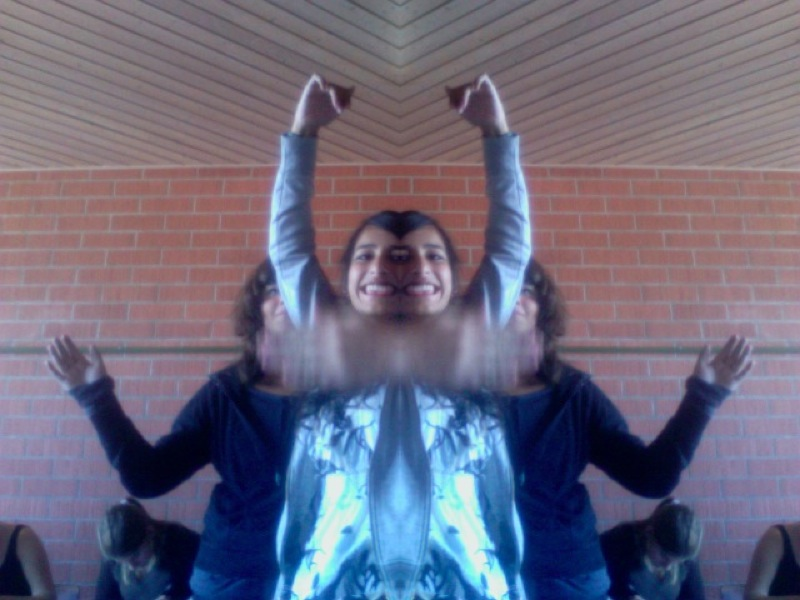
\includegraphics[width=0.618\textwidth]{miriam}}
\title{Affine Abbildungen}
\subtitle{Expectation vs. Reality}
\author{}
\date{}
%\lowertitleback{
%\includegraphics[height=1.1cm]{/Users/jormawassmer/Pictures/logokoeniz.jpg}%
%\copyright Jorma Wassmer
%1. Auflage, Februar 2011
%}


\begin{document}
\maketitle
\tableofcontents
%\thispagestyle{empty}
\cleardoublepage
%\setcounter{page}{1}

\section{Der Begriff der Abbildung}

\begin{wrapfigure}{r}{0.382\textwidth}
\vspace{-15pt}
  \begin{center}
    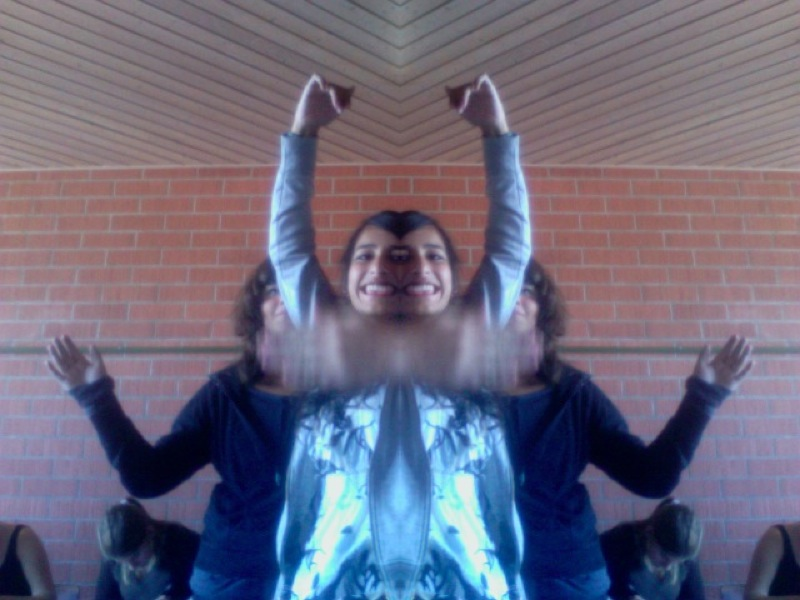
\includegraphics[width=0.382\textwidth]{miriam}
  \end{center}
%\caption{A gull}
\vspace{-22pt}
\end{wrapfigure}
Zunächst soll hier auf den allgemeinen Abbildungsbegriff eingegangen werden. Die weiteren Kapitel werden sich dann mit dem eigentlichem Thema befassen, den Abbildungen und im speziellen den affinen Abbildungen einer Ebene.

\subsection{Aus der Mengenlehre}
Personen oder auch Dinge stehen oft in Beziehung. Es gibt verwandtschaftliche oder freundschaftliche Beziehungen. Es gibt Beziehungen von Menschen zu ihrer Heimat, von Eigentümern zu ihrem Besitztum, oder auch zwischen Konjunktur und Arbeitslosigkeit, zwischen Qualität und Preis etc.

Manche Beziehungen lassen sich graphisch darstellen und mathematisch beschreiben. Im Folgenden werden Menge und Beziehungen zwischen ihren Elementen betrachtet.

\begin{bsp}
Es gibt eine Beziehung, in der Mathematik sagt man Relation, zwischen den Mitgliedern dieser Klasse und den mäglichen Freifächern, welche Angeboten werden.
\end{bsp}

\begin{cdef}
Unter einer \textbf{Relation} $R$ zwischen den Elementen der Mengen $\mA$ und $\mB$ versteht man eine beliebige Beziehung (Zuordnung), wodurch jedem Element $x\in\mA$ kein, genau ein oder mehr als ein Element $y\in\mB$ zugeordnet wird. Man schreibt
$$R:\mA\longrightarrow\mB$$
\end{cdef}

\begin{bsp}
Im obigen Beispiel steht $R$ für \glqq zu einem Klassenmitglied das Freifach zuordnen, $\mA$ für die Menge der Schülerinnen und Schüler der Klasse und $\mB$ für die Menge der angebotenen Freifächer.
\end{bsp}

\begin{bem}
Offensichtlich kann jede Relation als Menge von geordneten Paaren $\point{x}{y}$ notiert werden. Damit lässt sich der Relationsbegriff auch rein Mengentheoretisch definieren, nämlich via Produktmengen.
\end{bem}

\subsection{Produktmenge}
\begin{cdef}
Die \textbf{Produktmenge} zweier Mengen $\mA$ und $\mB$ besteht aus sämtlichen geordneten Paaren $\point{x}{y}$ mit $x\in\mA$ und $y\in\mB$. Man schreibt
$$\mA\times\mB=\setm{\point{x}{y}}{x\in\mA\text{ und }y\in\mB}$$
(lies \glqq A kreuz B\grqq)
\end{cdef}

\begin{bsp}
Sind $\mA=\set{1,2}$ und $\mB=\set{a,b,c}$, dann ist ihre Produktmenge
$$\mA\times\mB=\set{(1,a),(1,b),(1,c),(2,a),(2,b),(2,c)}.$$
\end{bsp}

\begin{ueb}
Ermitteln Sie die Mengen $\D{A}$ und $\D{B}$, falls
$$\D{A}\times\D{B}=\set{(3,1),(3,2),(6,1),(6,2),(9,1),(9,2)}$$
\end{ueb}

\subsection{Relation}

\begin{cdef}
Eine \textbf{Relation} $R$ zwischen den Elementen der Mengen $\mA$ und $\mB$ ist eine Teilmenge der Produktmenge $\mA\times\mB$.
\end{cdef}

\begin{bem}
Falls die Mengen $\mA$ und $\mB$ Zahlenmengen sind, kännen die Paare $\point{x}{y}$ als Punkte in einem rechtwinkligen Koordinatensystem veranschaulicht werden.

Die Darstellung der Relationen in einem rechtwinkligen Koordinatensystem nennt man das \textbf{Bild} der Relation.
\end{bem}

\subsection{Abbildung}

\begin{cdef}
Unter einer \textbf{Abbildung} $\ga$ einer Menge $\mA$ in eine Menge $\mB$ wird eine Zuordnung verstanden, die jedem Element $x\in\mA$ genau ein Element $x'\in\mB$ zuordnet
\footnote{
In der Analysis heissen Abbildungen meist Funktionen, nämlich dann, wenn die Wertemenge eine Zahlenmenge ist. Sie werden üblicherweise mit lateinischen Kleinbuchstaben wie $f, g$ etc. bezeichnet. Das einem $x$ zugeordnete Element wird dann als $y$ oder, wenn die Zuordnung $f$ heisst, als $f(x)$ geschrieben. In der Geometrie hingegen ist es üblich, eine Abbildung mit einem griechischen Kleinbuchstaben zu bezeichnen (z.B. $\ga$).
}.
$\ga(x)=x'$ heisst dann das \textbf{Bild} von $x$ und $x$ ist ein \textbf{Urbild} von $x'$.
\end{cdef}

Ein Element aus $\mB$ kann kein Urbild, ein Urbild oder mehrere Urbilder haben; in diesem Zusammenhang werden drei spezielle Eigenschaften von Abbildungen unterschieden:

\begin{itemize}
\item Eine Abbildung heisst \textbf{injektiv}, wenn verschiedene Elemente aus $\mA$ verschiedene Bilder haben, mit anderen Worten: Wenn jedes Element in $\mB$ \emph{hächstens} ein Urbild hat.
\item Hat jedes Element aus $\mB$ \emph{mindestens} ein Urbild, so spricht man von einer \textbf{surjektiven} Abbildung.
\item Hat jedes Element aus $\mB$ \emph{genau ein} Urbild, so handelt es sich um eine eineindeutige Abbildung von $\mA$ auf $\mB$. Eine solche Abbildung heisst auch \textbf{bijektiv}.
\end{itemize}

\begin{csatz}
Eine Abbildung ist genau dann bijektiv, wenn sie surjektiv und injektiv ist.
\end{csatz}

\begin{proof}[Beweis]
trivial
\end{proof}

\begin{bsp}
Betrachte die Abbildung $f(x) = x^2$. Je nach Einschränkung des Definitions-
und/oder des Bildbereiches kännen verschiedene Situationen kreiert werden.

\begin{itemize}
\item $f_1:\mR\longrightarrow\mR$
\item $f_2:\mR^+_0\longrightarrow\mR$
\item $f_3:\mR\longrightarrow\mR^+_0$
\item $f_4:\mR^+_0\longrightarrow\mR^+_0$
\end{itemize}
\end{bsp}

\begin{bem}
Jede Funktion kann problemlos, d.h. ohne Einschränkung der Funktion, zu einer surjektiven gemacht werden, indem die \glqq überflüssigen\grqq\ Elemente aus der Bildmenge gestrichen werden. Bei nicht injektiven geht das nicht ohne die Funktion zu beeinträchtigen.
\end{bem}

Oft ist es so, dass die Menge $\mB$ mit $\mA$ zusammenfällt. Man spricht dann von einer Abbildung der Menge A in sich.
Die meisten Funktionen, die du bis jetzt in der Analysis angetroffen hast, sind Abbildungen von Zahlenmengen (meist $\mR$) in sich. In der Geometrie sind Verschiebung, Spiegelung oder Drehung einer Ebene so geartete Abbildungen. Es sind Abbildungen vom $\mR^2$ in sich.

Eine spezielle Abbildung einer Menge $\mA$ in sich ist die so genannte \textbf{Identität}. Sie führt jedes Element in sich selbst über. Sie wird mit $\ge$ oder häufig allgemein als $\id$ bezeichnen. Es ist die Abbildung bei der nichts passiert, also alles beim Alten bleibt.

\subsection{Verknüpfung und Inverse}

\begin{cdef}
Werden zwei Abbildungen $\ga:\mA\longrightarrow\mB$ und $\gb:\mB\longrightarrow\mC$ hintereinander ausgeführt, so spricht man von einer \textbf{Verknüpfung} zweier Abbildungen. Es resultiert eine neue Abbildung $\gg:\mA\longrightarrow\mC$. Geschrieben:
$$\gg=\gb\circ\ga$$
(Beachte die Reihenfolge!).
\end{cdef}

Ist $\ga$ eine bijektive Abbildung von $\mA$ nach $\mB$, so hat gemäss Definition jedes Element aus $\mB$ genau ein Urbild. Es muss damit auch mäglich sein, eine neue, \glqq umgekehrte\grqq\ Abbildung von $\mB$ nach $\mA$ zu definieren, die jedem Bild der Abbildung $\ga$ sein Urbild zuordnet. Eine solche Abbildung heisst \textbf{inverse} Abbildung oder Umkehrabbildung von $\ga$ und wird mit $\ga^{-1}$ oder $\bar{\ga}$ bezeichnet.

\begin{satz}
Ist $\ga$ eine bijektive Abbildung so gilt:
$$\ga^{-1}\circ\ga=\id.$$
\end{satz}

\begin{proof}[Beweis]
trivial
\end{proof}

\begin{bsp}
\label{bsp:inverse}
Die Funktion $f(x) = 2x + 6$ ist eine bijektive Abbildung; sie besitzt also eine
Umkehrabbildung, nämlich $f^{-1}(x)=\frac{1}{2}x-3$.
\end{bsp}

\begin{ueb}
Bestätige rechnerisch Beispiel \ref{bsp:inverse}.
\end{ueb}

\begin{ueb}
Die Abbildung $\ga$ bezeichne eine Drehung der Ebene um $30^\circ$ um einen Punkt $Z$. Auch diese Abbildung ist bijektiv. Die Umkehrabbildung $\ga^{-1}$ ist dann\dots
\end{ueb}

\begin{ueb}
Die Funktion $f(x) = \frac{1}{2}x^2-4x+3$ soll auf einem mäglichst grossen Bereich umgekehrt werden.
\end{ueb}

\begin{ueb}\label{uebinjsurbij}
\ \\[-4ex]
\begin{enumeratea}
\item Es sei $\mA$ und $\mB$ die Menge der ganzen Zahlen. Die Abbildung $f$ führe jede Zahl in ihr Doppeltes über. Die Abbildung $f$\dots
\item Es sei $\mA$ und $\mB$ die selbe Ebene. Die Abbildung $\ga$ bezeichne die Verknüpfung einer zentrische Streckung mit dem Faktor $2$ von einen Punkt $Z$ aus und einer Verschiebung (Translation) um den Vektor $\vc$. Die Abbildung $\ga$\dots

(i) ist injektiv,$\q$(ii) surjektiv,$\q$(iii) bijektiv,$\q$(iv) besitzt eine inverse Abbildung?
\end{enumeratea}
\end{ueb}

\pagebreak

\begin{ueb}
Wie Übung \ref{uebinjsurbij}:

\begin{enumeratea}
\addtocounter{enumi}{2}
\item $g(x)=x+3$, mit $\mA=\mB=\mR$,
\item $h(x)=x^2$, mit $\mA=\mR$ und $\mB=\mR^+_0$,
\item $i(x)=\sqrt{x}$, mit $\mA=\mR^+_0$ und $\mB=\mR$,
\item $j(x)=\frac{1}{x}$, mit $\mA=\mR^*$ und $\mB=\mR^*$,
\item $\gb:$ Projektion der Ebene auf die x-Achse,
\item $\gg:\va\mapsto\frac{1}{\abs{\va}^2}\cdot\va$ (Inversion am Einheitskreis)
\end{enumeratea}
\end{ueb}

\begin{ueb}
Kann bei den oben beschriebenen Aufgaben der Definitions- oder der Bildbereich so ein- geschränkt werden, das bijektive Abbildungen entstehen?
\end{ueb}

\section{Abbildungen in der Ebene}

\begin{wrapfigure}{r}{0.382\textwidth}
\vspace{-15pt}
\centering
\definecolor{qqqqff}{rgb}{0,0,1}
\definecolor{zzttqq}{rgb}{0.6,0.2,0}
\scalebox{1}{
\begin{tikzpicture}[line cap=round,line join=round,>=triangle 45,x=0.5cm,y=0.5cm]
\clip(-6.34,-0.42) rectangle (5.42,5.34);
\fill[color=zzttqq,fill=zzttqq,fill opacity=0.1] (-2.6,4.96) -- (4.9,4.5) -- (2.36,0.54) -- (-6.06,1.66) -- cycle;
\draw [color=zzttqq] (-2.6,4.96)-- (4.9,4.5);
\draw [color=zzttqq] (2.36,0.54)-- (-6.06,1.66);
\draw [color=zzttqq] (-6.06,1.66)-- (-2.6,4.96);
\draw [shift={(-1.42,6.02)}] plot[domain=4.46:5.57,variable=\t]({1*4.23*cos(\t r)+0*4.23*sin(\t r)},{0*4.23*cos(\t r)+1*4.23*sin(\t r)});
\draw [->] (1.56,3.02) -- (1.78,3.26);
\draw (2.06,1.5) node[anchor=north] {$E$};
\fill [color=qqqqff] (-2.48,1.92) circle (1.5pt);
\draw[color=qqqqff] (-2.34,2.18) node[anchor=south]  {$P$};
\fill [color=qqqqff] (1.78,3.26) circle (1.5pt);
\draw[color=qqqqff] (1.96,3.52) node[anchor=south]  {$P'$};
\draw[color=black] (-0.16,2.32) node {$\ga$};
\end{tikzpicture}
}
\caption{Abbildung einer Ebene in sich}
\end{wrapfigure}
Im Folgenden werden ausschliesslich Abbildungen einer Ebene $E$ in sich betrachtet. Vorausgesetzt sei zudem, dass in $E$ ein (kartesisches) Koordinatensystem definiert ist.
\begin{cdef}
Unter
\marginnote{
\qrcode{
https://www.youtube.com/watch?v=zuHJopS96eo}
}
einer \textbf{Abbildung einer Ebene $E$ in sich} versteht man eine Zuordnung, die jedem Punkt $P\in E$ einen weiteren Punkt $P'\in E$ (das Bild von P) zuordnet. Sind $x$ und $y$ die Koordinaten eines Punktes $P$, so werden diejenigen seines Bildes $P'$ mit $x'$ und $y'$ bezeichnet.
\end{cdef}
An ein paar Beispielen soll jetzt erst mal gezeigt werden, wie Abbildungen von $E$ in sich mit rechnerischen Mitteln erfasst werden kännen.

\subsection{Zentrische Streckung vom Ursprung aus}
Die
\marginnote{
\qrcode{
https://www.youtube.com/watch?v=0hj4DWt-PQo}
}
Streckung $\ga$ mit dem Zentrum in $O$ und dem Faktor $k\neq0$ kann folgendermassen beschrieben werden:

Jedem Punkt $P\in E$ wird derjenigen Punkt $P'\in E$ zugeordnet, für den gilt:
$$\V{OP'}=k\cdot\V{OP}.$$
Der Ortsvektor
$$\V{r'}=\V{OP'}=\pv{x'}{y'}$$
von $P'$ ergibt sich, indem der Ortsvektor
$$\V{r}=\V{OP}=\pv{x}{y}$$
von $P$ mit $k$ multipliziert wird. Die Abbildungsgleichung $\ga$ kann damit durch ein einfaches System zweier linearer Gleichungen wiedergegeben werden:
$$\ga:
\begin{cases}
\;x'= kx \\
\;y'=&ky
\end{cases}
$$

\begin{figure}[h]
\centering
\definecolor{uququq}{rgb}{0.25,0.25,0.25}
\definecolor{zzttqq}{rgb}{0.6,0.2,0}
\definecolor{qqqqff}{rgb}{0,0,1}
\scalebox{1.2}{
\begin{tikzpicture}[line cap=round,line join=round,>=triangle 45,x=0.5cm,y=0.5cm]
\draw[->,color=black] (-2.22,0) -- (10.08,0);
\foreach \x in {-2,-1,1,2,3,4,5,6,7,8,9}
\draw[shift={(\x,0)},color=black] (0pt,2pt) -- (0pt,-2pt);
\draw[color=black] (9.74,0.08) node [anchor=south west] {$x$};
\draw[->,color=black] (0,-1.3) -- (0,8.46);
\foreach \y in {-1,1,2,3,4,5,6,7,8}
\draw[shift={(0,\y)},color=black] (2pt,0pt) -- (-2pt,0pt);
\draw[color=black] (0.1,8.06) node [anchor=west] {$y$};
\clip(-2.22,-1.3) rectangle (10.08,8.46);
\fill[color=zzttqq,fill=zzttqq,fill opacity=0.1] (-0.74,2.7) -- (3.66,3.78) -- (4.44,1.96) -- cycle;
\fill[color=zzttqq,fill=zzttqq,fill opacity=0.1] (-1.48,5.4) -- (7.32,7.56) -- (8.88,3.92) -- cycle;
\draw [color=zzttqq] (-0.74,2.7)-- (3.66,3.78);
\draw [color=zzttqq] (3.66,3.78)-- (4.44,1.96);
\draw [color=zzttqq] (4.44,1.96)-- (-0.74,2.7);
\draw [color=zzttqq] (-1.48,5.4)-- (7.32,7.56);
\draw [color=zzttqq] (7.32,7.56)-- (8.88,3.92);
\draw [color=zzttqq] (8.88,3.92)-- (-1.48,5.4);
\draw [->] (0,0) -- (4.44,1.96);
\draw [->] (4.44,1.96) -- (8.88,3.92);
\draw [dash pattern=on 1pt off 1pt] (-1.48,5.4)-- (0,0);
\draw [dash pattern=on 1pt off 1pt] (0,0)-- (7.32,7.56);
\fill [color=qqqqff] (-0.74,2.7) circle (1.5pt);
\draw[color=qqqqff] (-1.04,2.78) node[anchor=east] {$R$};
\fill [color=qqqqff] (3.66,3.78) circle (1.5pt);
\draw[color=qqqqff] (3.46,4.14) node {$Q$};
\fill [color=qqqqff] (4.44,1.96) circle (1.5pt);
\draw[color=qqqqff] (4.54,1.58) node[anchor=north]  {$P$};
\fill [color=uququq] (0,0) circle (1.5pt);
\draw[color=uququq] (-0.34,-0.32) node[anchor=north east]  {$O$};
\fill [color=qqqqff] (-1.48,5.4) circle (1.5pt);
\draw[color=qqqqff] (-1.5,5.82) node[anchor=south] {$R'$};
\fill [color=qqqqff] (7.32,7.56) circle (1.5pt);
\draw[color=qqqqff] (7.08,7.92) node {$Q'$};
\fill [color=qqqqff] (8.88,3.92) circle (1.5pt);
\draw[color=qqqqff] (8.9,3.48) node[anchor=north]  {$P'$};
\draw[color=black] (2.22,1.2) node[anchor=south west]  {$r$};
\draw[color=black] (6.7,3.16) node[anchor=south west]  {$r'$};
\end{tikzpicture}
}
\caption{Zentrische Streckung am Ursprung mit Faktor $k=2$}
\end{figure}

\begin{ueb}
$\ga$ sei die Streckung mit dem Zentrum $O$ und dem Streckungsfaktor $\frac{3}{2}$.
\begin{enumeratea}
\item Wie heissen die Abbildungsgleichungen von $\ga$?
\item Bestimme das Bild des Punktes $P = \point{2}{6}$.
\item Bestimme das Urbild von $Q'=\point{4.5}{-2.1}$.
\item Bestimme die Gleichungen der Umkehrabbildung $\ga^{-1}$.
\end{enumeratea}
\end{ueb}

\subsection{Translation}
Eine Verschiebung $\gt$ in der Ebene um einen Vektor $\vv$ kann folgendermassen beschrieben werden:

Jedem Punkt $P\in E$ wird derjenigen Punkt $P'\in E$ zugeordnet, für den gilt:
$$\V{OP'}=\V{OP}+\vv.$$

\begin{figure}[h]
\centering
\definecolor{zzttqq}{rgb}{0.6,0.2,0}
\definecolor{qqqqff}{rgb}{0,0,1}
\scalebox{1}{
\begin{tikzpicture}[line cap=round,line join=round,>=triangle 45,x=0.5cm,y=0.5cm]
\draw[->,color=black] (-2.42,0) -- (10.3,0);
\foreach \x in {-2,-1,1,2,3,4,5,6,7,8,9,10}
\draw[shift={(\x,0)},color=black] (0pt,2pt) -- (0pt,-2pt);
\draw[color=black] (9.96,0.08) node [anchor=south west] {$x$};
\draw[->,color=black] (0,-0.8) -- (0,7.16);
\foreach \y in {1,2,3,4,5,6}
\draw[shift={(0,\y)},color=black] (2pt,0pt) -- (-2pt,0pt);
\draw[color=black] (0.1,6.76) node [anchor=west] {$y$};
\clip(-2.42,-0.8) rectangle (10.3,7.16);
\fill[color=zzttqq,fill=zzttqq,fill opacity=0.1] (-1.24,1.82) -- (2.8,0.58) -- (2,4) -- cycle;
\fill[color=zzttqq,fill=zzttqq,fill opacity=0.1] (4.72,4.14) -- (8.76,2.9) -- (7.96,6.32) -- cycle;
\draw [color=zzttqq] (-1.24,1.82)-- (2.8,0.58);
\draw [color=zzttqq] (2.8,0.58)-- (2,4);
\draw [color=zzttqq] (2,4)-- (-1.24,1.82);
\draw [->] (2.8,0.58) -- (8.76,2.9);
\draw [color=zzttqq] (4.72,4.14)-- (8.76,2.9);
\draw [color=zzttqq] (8.76,2.9)-- (7.96,6.32);
\draw [color=zzttqq] (7.96,6.32)-- (4.72,4.14);
\draw [dash pattern=on 1pt off 1pt] (2.8,0.58)-- (8.76,0.58);
\draw [dash pattern=on 1pt off 1pt] (8.76,2.9)-- (8.76,0.58);
\fill [color=qqqqff] (-1.24,1.82) circle (1.5pt);
\draw[color=qqqqff] (-1.34,1.44) node[anchor=east]  {$R$};
\fill [color=qqqqff] (2.8,0.58) circle (1.5pt);
\draw[color=qqqqff] (2.8,0.3) node[anchor=east] {$P$};
\fill [color=qqqqff] (2,4) circle (1.5pt);
\draw[color=qqqqff] (2.16,4.1) node[anchor=south]  {$Q$};
\draw[color=black] (5.66,2.06) node {$\vv$};
\fill [color=qqqqff] (4.72,4.14) circle (1.5pt);
\draw[color=qqqqff] (4.66,3.7) node {$R'$};
\fill [color=qqqqff] (8.76,2.9) circle (1.5pt);
\draw[color=qqqqff] (9.3,3) node {$P'$};
\fill [color=qqqqff] (7.96,6.32) circle (1.5pt);
\draw[color=qqqqff] (8.16,6.58) node[anchor=west]  {$Q'$};
\end{tikzpicture}
}
\caption{Translation mit dem Vektor $\vv$}
\end{figure}

Besitzt der Verschiebungsvektor die Komponenten $\pv{v_x}{v_y}$, so ergibt sich für die Abbildungsgleichung $\gt$ das Gleichungssystem:
$$\glsys{\gt}{x&\phantom{y}+v_x}{&y+v_y}$$

\begin{ueb}
Gegeben sei die Translation
$$\glsys{\gt}{x&\phantom{y}+1}{&y-2}$$
\begin{enumeratea}
\item Handelt es sich bei $\gt$ um eine Bijektion? Begründe.
\item Gib die Umkehrabbildung $\gt^{-1}$ an.
\item Wird eine Streckung $\ga$ mit einer Verschiebung $\gt$ verknüpft, so entsteht eine neue Abbildung. Ist die Verknüpfung kommutativ, d.h. gilt
$$\ga\circ\gt=\gt\circ\ga?$$
Gib die Abbildungsgleichungen der beiden Verknüpfungsarten $\ga\circ\gt$ bzw. $\gt\circ\ga$ an, wobei $\ga$ die Streckung am Ursprung um den Faktor $k = 3$ und $\gt$ die oben definierte Translation sein soll.
\item Wie lauten die Abbildunsgleichungen einer Streckung mit dem Zentrum $S=(1|5)$ und dem Streckungsfaktor $k = 3$?

Bestimme das Bild von $O=\point{0}{0}$ und $P =\point{2}{-3}$ sowie das Urbild von $Q' =\point{-5}{8}$.
\item Allgemein: Wie lauten die Abbildunsgleichungen einer Streckung mit Zentrum $S =\point{s_x}{s_y}$ und dem Streckungsfaktor $k$?
\end{enumeratea}
\end{ueb}

\subsection{Spiegelung an den Koordinatenachsen}
Soll an einer Koordinatenachse gespiegelt werden, zum Beispiel an der $x$-Achse, so ändert einfach das Vorzeichen der entsprechenden Koordinate, also hier der $y$-Koordinate. Für die Abbildungsgleichung $\ga$ ergibt sich dann das Gleichungssystem:
$$\glsysa{x}{&-y}$$
Wird an der $y$-Achse gespiegelt, so ergibt sich das Gleichungssystem:
$$\glsys{\gb}{-x}{&y}$$

\begin{ueb}
\ \\[-4ex]
\begin{enumeratea}
\item Wie lauten die Umkehrabbildungen von $\ga$ und $\gb$?
\item Was für eine Abbildung ergibt sich bei einer Verknüpfung der beiden Achsenspiegelungen und wie lauten ihre Gleichungen?
\item\label{item:gerade} Wie lauten die Abbildungsgleichungen der Spiegelung an der zur $y$-Achse parallelen Geraden $g: x = 2$ (allgemein: an der Geraden $x = a$)?
\item Spiegle zuerst an der Geraden $h: y = -1$ und anschliessend an $g$ aus Aufgabe \eqref{item:gerade}. Was für ein Abbildungstyp resultiert? Wie lauten die Abbildungsgleichungen?
\item Gib die Abbildungsgleichungen einer Punktspiegelung am Punkt $\point{s_x}{s_y}$ an.
\item Verknüpfe eine Achsen- mit einer Punktspiegelung am Ursprung (in dieser Reihenfolge). Was ergibt sich? Gib die Abbildungsgleichungen an.
\item Gib die Abbildungsgleichungen $\gb\circ\ga$ an, die bei der Verknüpfung der Streckung $\ga$ am Ursprung um den Faktor $-2$ und der Spiegelung $\gb$ an der x-Achse entstehen.
\end{enumeratea}
\end{ueb}

\subsection{Scherung an der Koordinatenachse}
Untersuche die Abbildung $\gg$ gegeben durch
$$\glsys{\gg}{\phantom{\frac{3}{2}}x}{\frac{3}{2}x&+y}$$
indem du die Urbilder und Bilder von verschiedenen Punkten ins Koordinatenystem (auf Seite \pageref{bilderundurbilder}) einzeichnest und die Abbildung so analysierst.

\begin{figure}
\begin{center}
\definecolor{cqcqcq}{rgb}{0.75,0.75,0.75}
\begin{tikzpicture}[line cap=round,line join=round,>=triangle 45,x=1cm,y=1cm]
\draw [color=cqcqcq,dash pattern=on 2pt off 2pt, xstep=1cm,ystep=1cm] (-4.5,-3.5) grid (6.5,6.5);
\draw[->,color=black] (-4.5,0) -- (6.5,0);
\foreach \x in {-4,-3,-2,-1,1,2,3,4,5,6}
\draw[shift={(\x,0)},color=black] (0pt,2pt) -- (0pt,-2pt) node[below] {\footnotesize $\x$};
\draw[color=black] (6.14,0.09) node [anchor=south west] {$x$};
\draw[->,color=black] (0,-3.5) -- (0,6.5);
\foreach \y in {-3,-2,-1,1,2,3,4,5,6}
\draw[shift={(0,\y)},color=black] (2pt,0pt) -- (-2pt,0pt) node[left] {\footnotesize $\y$};
\draw[color=black] (0.1,6.05) node [anchor=west] {$y$};
\draw[color=black] (0pt,-10pt) node[right] {\footnotesize $0$};
\clip(-4.5,-3.5) rectangle (6.5,6.5);
\end{tikzpicture}
\end{center}
\caption{Bilder und Urbilder von $\gg$}\label{bilderundurbilder}
\end{figure}

\begin{cdef}
Eine \textbf{Scherung} an der $x$-Achse kann durch einen so genannten Scherungswinkel $\varphi$ festgelegt werden. Er misst den Winkel zwischen einem abzubildenden Punkt $P$, seiner Projektion auf der $x$-Achse und dem Bildpunkt $P'$, und zwar im Uhrzeigersinn.
\end{cdef}

\begin{figure}
\centering
\definecolor{xdxdff}{rgb}{0.49,0.49,1}
\definecolor{qqwuqq}{rgb}{0,0.39,0}
\definecolor{qqqqff}{rgb}{0,0,1}
\scalebox{1.2}{
\begin{tikzpicture}[line cap=round,line join=round,>=triangle 45,x=0.5cm,y=0.5cm]
\draw[->,color=black] (-4.28,0) -- (7.02,0);
\foreach \x in {-4,-3,-2,-1,1,2,3,4,5,6}
\draw[shift={(\x,0)},color=black] (0pt,2pt) -- (0pt,-2pt);
\draw[color=black] (6.68,0.08) node [anchor=south west] {$x$};
\draw[->,color=black] (0,-3.44) -- (0,5.1);
\foreach \y in {-3,-2,-1,1,2,3,4}
\draw[shift={(0,\y)},color=black] (2pt,0pt) -- (-2pt,0pt);
\draw[color=black] (0.1,4.7) node [anchor=west] {$y$};
\clip(-4.28,-3.44) rectangle (7.02,5.1);
\draw [shift={(-3,0)},color=qqwuqq,fill=qqwuqq,fill opacity=0.1] (0,0) -- (56.31:1.1) arc (56.31:90:1.1) -- cycle;
\draw [shift={(2,0)},color=qqwuqq,fill=qqwuqq,fill opacity=0.1] (0,0) -- (56.31:1.1) arc (56.31:90:1.1) -- cycle;
\draw [shift={(5,0)},color=qqwuqq,fill=qqwuqq,fill opacity=0.1] (0,0) -- (-123.69:1.1) arc (-123.69:-90:1.1) -- cycle;
\draw [->] (-3,3) -- (-1,3);
\draw [->] (2,4) -- (4.66,3.99);
\draw [->] (5,-2) -- (3.66,-2.01);
\draw [dotted] (-3,3)-- (0.5,3);
\draw [dotted] (5,-2)-- (-0.5,-2);
\draw [dotted] (4.66,3.99)-- (-0.84,3.99);
\draw [dash pattern=on 1pt off 1pt] (-3,3)-- (-3,0);
\draw [dash pattern=on 1pt off 1pt] (-3,0)-- (-1,3);
\draw [dash pattern=on 1pt off 1pt] (2,4)-- (2,0);
\draw [dash pattern=on 1pt off 1pt] (2,0)-- (4.66,3.99);
\draw [dash pattern=on 1pt off 1pt] (5,-2)-- (5,0);
\draw [dash pattern=on 1pt off 1pt] (5,0)-- (3.66,-2.01);
\fill [color=qqqqff] (-1,3) circle (1.5pt);
\draw[color=qqqqff] (-0.84,3.26) node[anchor=south] {$Q'$};
\fill [color=qqqqff] (-3,3) circle (1.5pt);
\draw[color=qqqqff] (-2.86,3.26) node[anchor=south] {$Q$};
\draw[color=qqwuqq] (-2.75,0.8) node {$\varphi$};
\fill [color=qqqqff] (2,4) circle (1.5pt);
\draw[color=qqqqff] (2.14,4.26) node[anchor=south] {$P$};
\draw[color=qqwuqq] (2.25,0.8) node {$\varphi$};
\fill [color=xdxdff] (4.66,3.99) circle (1.5pt);
\draw[color=xdxdff] (4.82,4.26) node[anchor=south] {$P'$};
\fill [color=qqqqff] (5,-2) circle (1.5pt);
\draw[color=qqqqff] (5.16,-2.1) node[anchor=north] {$R$};
\draw[color=qqwuqq] (4.8,-0.75) node {$\varphi$};
\fill [color=xdxdff] (3.66,-2.01) circle (1.5pt);
\draw[color=xdxdff] (3.76,-2.1) node[anchor=north] {$R'$};
\end{tikzpicture}
}
\caption{Scherung an der $x$-Achse um den Winkel $\varphi$}
\end{figure}
\noindent Für die Abbildungsgleichung gilt dann:
$$\glsysa{x&+\;y\cdot\tan(\varphi)}{&\phantom{\;+}y}$$
Wird $k = \tan(\varphi)$ gesetzt, so ergibt das kurz:
$$\glsysa{x&+\;ky}{&\phantom{\;+k}y}$$
Analoge †berlegungen führen zur Scherung an der $y$-Achse (der Scherungswinkel wird dann allerdings im Gegenuhrzeigersinn gemessen):
$$\glsys{\gb}{\phantom{k}x}{kx&+y}$$

\begin{ueb}
\ \\[-4ex]
\begin{enumeratea}
\item\label{item:scherung} Wie lauten die Abbildungsgleichungen der Scherung an der $x$-Achse mit dem Scherungswinkel $\varphi = -60^\circ$?
\item Gib die Umkehrabbildung der in \eqref{item:scherung} gegebenen Scherung an.
\item Gib die Abbildungsgleichungen der Scherung an der zur $x$-Achse parallelen Geraden $g:y=2$ um den Winkel $\alpha$ an.
\end{enumeratea}
\end{ueb}

\begin{ueb}
Berechne die Bildpunkte von
$$A = \point{-3}{5}\q\text{und}\q B = \point{2}{11}$$
bei der
\begin{enumeratea}
\item\label{item:spiegelung} Spiegelung an der $y$-Achse,
\item Drehung um den Ursprung um $180^\circ$,
\item Drehung um den Ursprung im Gegenuhrzeigersinn um $90^\circ$,
\item\label{item:winkelhalbierende} Spiegelung an der Winkelhalbierenden der positiven $x$- und $y$-Achse.
\item Bestimme das Urbild von $P' = \point{-5}{15}$ unter den Abbildungen \eqref{item:spiegelung} bis \eqref{item:winkelhalbierende}.
\end{enumeratea}
\end{ueb}

\begin{ueb}\label{ueb:verketten}
Gegeben sind die Abbildungen
$$\glsysa{3x}{&3y}\qq\glsys{\gb}{-x&\phantom{y}-4}{&y}$$
und
$$\glsys{\gg}{-x&\phantom{-y}+6}{&-y+2}$$
\begin{enumeratea}
\item Um was für Abbildungen handelt es sich?
\item Gib die Abbildungsgleichungen der folgenden Verknüpfungen an:
\begin{enumeratei}
\item $\ga\circ\gb$
\item $\gb\circ\ga$
\item $\gg^{-1}$
\item $\gg\circ\gb$
\item $\gg\circ\gb\circ\gg^{-1}$
\end{enumeratei}
\end{enumeratea}
\end{ueb}

\begin{ueb}
Eine Scherung $\ga$ an der $x$-Achse bildet den Punkt $P =\point{3}{2}$ auf $P' =\point{5}{2}$ ab.
\begin{enumeratea}
\item Gib die Koordinaten der Bildpunkte von $Q=\point{2}{-1}$, $R=\point{-4}{6}$ und $S=\point{1}{3}$ an.
\item Stelle die Abbildungsgleichungen von $\ga$ auf.
\item Gib die Umkehrabbildung $\ga^{-1}$ dieser Scherung an.
\item Gib die Verknüpfung $\ga\circ\gg$ der Scherung $\ga$ mit der Abbildung $\gg$ aus \"Ubung \ref{ueb:verketten} an.
\item Kann die Verknüpfung einer Scherung an der $x$-Achse mit einer Scherung an der $y$-Achse wiederum eine Scherung oder gar eine Streckung ergeben?
\end{enumeratea}
\end{ueb}

\section{Bilder von Geraden}
Um
\marginnote{
\qrcode{
https://www.youtube.com/watch?v=V8tynQkpOW4}
}
eine Vorstellung von einer Abbildung zu bekommen, ist es häufig hilfreich nicht nur über die Bilder von einzelnen Punkten Bescheid zu wissen, sondern auch zu sehen, zu was beispielsweise eine Gerade transformiert wird. Insbesondere interessieren die Bilder der Koordinatenachsen.

\begin{ueb}
Eine Abbildung sei durch
$$\glsysa{x(1+y)}{y(1+x)}$$
gegeben.
\begin{enumeratea}
\item Berechne die Bildpunktkoordinaten des Ursprungs, von $E_1 = \point{1}{0}$, $E_2 = \point{0}{1}$, von $A=\point{a}{0}$, $B=\point{0}{b}$, $C_1 =\point{1}{1}$, $C_2 =\point{-1}{-1}$, $D_1 =\point{2}{2}$ und $D_2 =\point{-2}{-2}$.
\item Gib die Bilder der Koordinatenachsen an.
\item Wie lauten die Gleichungen der Bildgeraden $f_1 : y = 1$ und $f_2 : x = 1$?
\item Bestimme das Bild der Winkelhalbierenden $g : y = x$.
\item Es sieht so aus, wie wenn Geraden auf (Halb)Geraden abgebildet würden. Ist das tatsächlich so? Untersuche dazu das Bild der Geraden $h: y = 2x$.
\begin{center}
\definecolor{cqcqcq}{rgb}{0.75,0.75,0.75}
\begin{tikzpicture}[line cap=round,line join=round,>=triangle 45,x=0.7cm,y=0.7cm]
\draw [color=cqcqcq,dash pattern=on 1pt off 1pt, xstep=0.7cm,ystep=0.7cm] (-6.5,-4.5) grid (12.5,10.5);
\draw[->,color=black] (-6.5,0) -- (12.5,0);
\foreach \x in {-6,-4,-2,2,4,6,8,10,12}
\draw[shift={(\x,0)},color=black] (0pt,2pt) -- (0pt,-2pt) node[below] {\footnotesize $\x$};
\draw[color=black] (12.04,0.1) node [anchor=south west] {$x$};
\draw[->,color=black] (0,-4.5) -- (0,10.5);
\foreach \y in {-4,-2,2,4,6,8,10}
\draw[shift={(0,\y)},color=black] (2pt,0pt) -- (-2pt,0pt) node[left] {\footnotesize $\y$};
\draw[color=black] (0.14,9.98) node [anchor=west] {$y$};
\draw[color=black] (0pt,-10pt) node[right] {\footnotesize $0$};
\clip(-6.5,-4.5) rectangle (12.5,10.5);
\end{tikzpicture}
\end{center}
\end{enumeratea}
\end{ueb}

\begin{ueb}
Beantworte die unten stehenden Fragen für die folgenden Abbildungen:
$$\glsysa{3x&-\phantom{\;2}y}{\phantom{3}x&+\;2y}\qq\glsys{\gb}{-x&\phantom{+y}+1}{\phantom{-}x&+\;y}$$
und
$$\glsys{\gg}{x&\;-1}{x^2}$$
\begin{enumeratea}
\item Berechne die Bildpunktkoordinaten des Ursprungs, von $E_1 = \point{1}{0}$, $E_2 = \point{0}{1}$, von $A=\point{a}{0}$, $B=\point{0}{b}$, $C=\point{1}{1}$ und $D=\point{2}{-3}$.
\item Gib die Urbilder der Punkte $F' =\point{-2}{4}$, $G' =\point{5}{-3}$ und $H' =\point{2}{9}$ an.
\item Wie lauten die Umkehrabbildungen von $\ga$, $\gb$ und $\gg$?
\item Gib die Bilder der Koordinatenachsen an.
\item Wie lauten die Gleichungen der Bildgeraden $f_1 : y = 1$ und $f_2 : x = 1$?
\item Bestimme das Bild der Winkelhalbierenden $g : y = x$ und das Bild der Geraden
$h: y=2x-1$ rechnerisch.
\item Wird jede Gerade auf eine Gerade abgebildet?
\item Handelt es sich bei den Abbildungen um Bijektionen?
\end{enumeratea}
\end{ueb}

\section{Fixpunkte und Fixgeraden}
Bei
\marginnote{
\qrcode{
https://www.youtube.com/watch?v=RcQY8_7eHuI}
}
Abbildungen von Mengen in sich kann es vorkommen, dass Punkte oder gewisse Teilmengen auf sich selber abgebildet werden. Diese Punktmengen sind von einiger Bedeutung.

\begin{cdef}
Ein Punkt $P$, der bei einer Abbildung $\ga$ auf sich selber abgebildet wird, heisst \textbf{Fixpunkt} von $\ga$.
\end{cdef}

Es muss also gelten:
$$\ga(P)=P.$$

\begin{cdef}
Eine Gerade, die aus Fixpunkten einer Abbildung besteht, nennt man \textbf{Fixpunktgerade}. Eine Gerade $g : y = mx + b$ , die unter einer Abbildung $\ga$ auf sich selber --- nicht zwingend Punktweise --- abgebildet wird, wird als \textbf{Fixgerade} bezeichnet.
\end{cdef}

Für die Bildgerade $\ga(g)=g'$ mit $g' : y' = m'x' + b'$ muss demnach gelten:
$$m'=m\q\text{und}\q b'=b.$$

\begin{bsp}
Bei der Spiegelung an der $x$-Achse wird jeder Punkt der $x$-Achse auf sich selber abgebildet, er ist also Fixpunkt. Weil sich die Fixpunkte auf einer Geraden (hier der $x$-Achse) befinden, ist die $x$-Achse eine Fixpunktgerade und damit natürlich auch eine Fixgerade. Auch jede zur $y$-Achse parallele Gerade ist Fixgerade, aber keine Fixpunktgerade. Denn auf ihr wird nicht jeder Punkt auf sich abgebildet (nur der Schnittpunkt mit der $x$-Achse), aber immerhin bleibt das Bild jedes Punktes einer solchen Vertikalen auf ihr liegen.
\end{bsp}

\begin{ueb}
\ \\[-4ex]
\begin{enumeratea}
\item Bestimme die Fixpunkte der folgenden Abbildungen (ohne Rechnung):
\begin{quote}
Streckung, Translation, Scherung
\end{quote}
Existieren Fixgeraden oder gar Fixpunktgeraden?
\item Bestimme durch Rechnung die Fixpunkte und Fixgeraden der Abbildung
$$\glsysa{\phantom{2}x&+\;4y}{2x&-\;\phantom{4}y+8}$$
\item Eine Abbildung sei durch
$$\glsysa{x}{x^2&+\;y}$$
gegeben.
\begin{enumeratei}
\item Bestimme die Fixpunkte der Abbildung.
\item Zeige, dass alle zur $y$-Achse parallelen Geraden Fixgeraden sind.
\item Was passiert mit den zur $x$-Achse parallelen Geraden?
\item Zeige, dass keine weiteren Fixgeraden existieren.
\end{enumeratei}
\end{enumeratea}
\end{ueb}

\begin{ueb}
Bestimme die Fixpunkte und Fixgeraden der folgenden Abbildung:
\begin{align*}
&\glsys{\ga}{&\phantom{+\;}y}{x&+\;y}&\glsys{\gb}{2x&-\;y}{\phantom{2}x}\\[2ex]
&\glsys{\gg}{&4y}{9x}&\glsys{\gd}{\phantom{2}x&+\;1}{2x&-\;y}\\[2ex]
&\glsys{\ge}{\phantom{2}x&\phantom{+\;y}+1}{2x&+\;y}&\glsys{\gz}{5x&-\;y}{\phantom{5}\frac{1}{x}}
\end{align*}
\end{ueb}

\begin{ueb}
Die \textsc{Agnesi}-Abbildung
\footnote{
Die in dieser Aufgabe entstehende Kurve wurde in einem anderen Zusammenhang zuerst intensiv von der Mathematikerin \textsc{Maria Agnesi} (1718-1799) untersucht. Sie wird daher als \textsc{Agnesi}-Kurve bezeichnet. \textsc{Agnesi} wurde 1750 zur Professorin für Mathematik an die Universität Bologna berufen. Sie war, soweit heute bekannt, die erste Frau, die als Professorin Vorlesungen zur Mathematik an einer Universität hielt.
}
ist durch die Gleichungen
$$\glsysa{\frac{1}{1+x^2}}{&y}$$
definiert.
\begin{enumeratea}
\item Bestimme den Wertebereich von $\ga$.
\item Begr\"unde, dass eine zur $y$-Achse parallele Gerade auf eine zur $y$-Achse parallele Gerade abgebildet wird.
\item Zeige, dass es eine zur $y$-Achse parallele Fixpunktgerade gibt.
\item Bestimme das Bild einer zur $x$-Achse parallelen Geraden.
\item Skizziere das Bild der Winkelhalbierenden zwischen der $x$- und der $y$-Achse, indem du die Bildpunkte von mindestens 10 Punkten in ein Koordinatensystem einzeichnest.
\end{enumeratea}
\end{ueb}

\begin{ueb}
Die Inversion am Kreis ist durch die Gleichungen
$$\glsysa{\frac{x}{x^2+y^2}}{\frac{y}{x^2+y^2}}$$
definiert.
\begin{enumeratea}
\item Bestimme den Definitionsbereich von $\ga$.
\item Bestimme die Fixpunkte von $\ga$ und zeige, dass sie auf dem Einheitskreis mit Zentrum im Ursprung liegen.
\item Zeige, dass jede \glqq gelochte\grqq\ Ursprungsgerade (ohne Ursprung) eine Fixgerade ist.
\item Zeige, dass sich der Abstand eines Punktes $P$ zum Ursprung reziprok verhält zum Abstand des Bildpunktes $P'$ zum Ursprung:
$$\dist(O,P')=\frac{1}{\dist(O,P)}.$$
\item Mache dir mit Beispielen klar, dass das Bild der Geraden $y = 1$ gerade der \glqq gelochten\grqq\ Kreislinie
$$k : x^2 + (y-0.5)^2 = 0.5^2$$
(ohne Ursprung) entspricht.
\end{enumeratea}
\end{ueb}

\newpage

\section{Eigenschaften affiner Abbildungen}

\begin{center}
\definecolor{qqwuqq}{rgb}{0,0.39,0}
\definecolor{zzttqq}{rgb}{0.6,0.2,0}
\definecolor{qqqqff}{rgb}{0,0,1}
\begin{tikzpicture}[line cap=round,line join=round,>=triangle 45,x=0.7cm,y=0.7cm]
\clip(-3.72,-5.54) rectangle (4.66,5.52);
\fill[color=zzttqq,fill=zzttqq,fill opacity=0.1] (-2.76,-2.9) -- (-0.36,-4.98) -- (3.74,-1.58) -- cycle;
\fill[color=zzttqq,fill=zzttqq,fill opacity=0.1] (-0.32,-1.86) -- (1.76,0.54) -- (-1.64,4.64) -- cycle;
\draw [shift={(-2.06,-1.16)},color=qqwuqq] (0,0) -- (-111.91:0.9) arc (-111.91:-21.91:0.9) -- cycle;
\draw [color=zzttqq] (-2.76,-2.9)-- (-0.36,-4.98);
\draw [color=zzttqq] (-0.36,-4.98)-- (3.74,-1.58);
\draw [color=zzttqq] (3.74,-1.58)-- (-2.76,-2.9);
\draw [color=zzttqq] (-0.32,-1.86)-- (1.76,0.54);
\draw [color=zzttqq] (1.76,0.54)-- (-1.64,4.64);
\draw [color=zzttqq] (-1.64,4.64)-- (-0.32,-1.86);
\draw [shift={(-2.06,-1.16)},dash pattern=on 2pt off 2pt,color=zzttqq]  (0,0) --  plot[domain=4.33:5.9,variable=\t]({1*1.88*cos(\t r)+0*1.88*sin(\t r)},{0*1.88*cos(\t r)+1*1.88*sin(\t r)}) -- cycle ;
\draw [shift={(-2.06,-1.16)},dash pattern=on 2pt off 2pt,color=zzttqq]  (0,0) --  plot[domain=-1.15:0.42,variable=\t]({1*4.18*cos(\t r)+0*4.18*sin(\t r)},{0*4.18*cos(\t r)+1*4.18*sin(\t r)}) -- cycle ;
\draw [shift={(-2.06,-1.16)},dash pattern=on 2pt off 2pt,color=zzttqq]  (0,0) --  plot[domain=-0.07:1.5,variable=\t]({1*5.82*cos(\t r)+0*5.82*sin(\t r)},{0*5.82*cos(\t r)+1*5.82*sin(\t r)}) -- cycle ;
\fill [color=qqqqff] (-2.76,-2.9) circle (1.5pt);
\draw[color=qqqqff] (-2.7,-2.64) node[anchor=east] {$A$};
\fill [color=qqqqff] (-0.36,-4.98) circle (1.5pt);
\draw[color=qqqqff] (-0.22,-4.9) node[anchor=north] {$B$};
\fill [color=qqqqff] (3.74,-1.58) circle (1.5pt);
\draw[color=qqqqff] (3.9,-1.5) node[anchor=west] {$C$};
\fill [color=qqqqff] (-2.06,-1.16) circle (1.5pt);
\draw[color=qqqqff] (-2.44,-0.9) node {$Z$};
\fill [color=qqqqff] (-0.32,-1.86) circle (1.5pt);
\draw[color=qqqqff] (-0.76,-1.99) node {$A'$};
\fill [color=qqqqff] (1.76,0.54) circle (1.5pt);
\draw[color=qqqqff] (1.94,0.8) node[anchor=west] {$B'$};
\fill [color=qqqqff] (-1.64,4.64) circle (1.5pt);
\draw[color=qqqqff] (-1.46,4.9) node[anchor=south] {$C'$};
\draw[color=qqwuqq] (-1.9,-1.7) node {$\varphi$};
\end{tikzpicture}
\end{center}

\begin{ueb}
\ \\[-4ex]
\begin{enumeratea}
\item Durch welche Abbildung $\ga$ wird das Dreieck $ABC$ auf das Dreieck $A'B'C'$ abgebildet?
\item Welche Abbildung bildet das Dreieck $A'B'C'$ auf das Dreieck $ABC$ ab?
\item Bestimme das Bild der Geraden $g_{AB}$.
\item Auf welchen Punkt wird der Mittelpunkt der Strecke $\overline{AB}$ abgebildet?
\item Kännen sich die Bilder zweier zueinander paralleler Geraden schneiden?
\end{enumeratea}
\end{ueb}

Viele geometrische Abbildungen, die uns bis jetzt begegnet sind, besitzen die folgenden Eigenschaften:
\begin{itemize}
\item Sie sind \textbf{geradentreu}, d.h. sie bilden Geraden auf Geraden ab.
\item Sie sind \textbf{umkehrbar} (bijektiv), d.h. zu jedem Bildpunkt existiert genau ein Urbild.
\item Sie sind \textbf{parallelentreu}, d.h. sie bilden zueinander parallele Geraden auf zueinander parallele Geraden ab.
\item Sie sind \textbf{teilverhältnistreu}: Wenn ein Punkt $T$ eine Strecke $\overline{AB}$ im Verhältnis $t$ teilt, so teilt auch sein Bildpunkt $T'$ die Bildstrecke $\overline{A'B'}$ im Verhältnis $t$.
\end{itemize}

\begin{satz}
Geradentreue, umkehrbare Abbildungen sind parallelentreu und teilverhältnistreu.
\end{satz}

\begin{proof}[Beweis]
Aus der Umkehrbarkeit einer geradentreuen Abbildung folgt ihre Parallelentreue. Hätten nämlich die Bilder zweier (verschiedener) paralleler Geraden $g$ und $h$ einen Schnittpunkt, dann müsste dieser Schnittpunkt zwei Urbilder haben, nämlich einen auf $g$ und einen auf $h$. Aber das kann wegen der Umkehrbarkeit nicht sein.

Aufgrund der Parallelentreue bildet jede geradentreue, umkehrbare Abbildung Parallelogramme auf Parallelogramme ab. Damit wird der Mittelpunkt einer Strecke $\overline{AB}$ auf den Mittelpunkt der Bildstrecke $\overline{A'B'}$ abgebildet. Mit Hilfe einer Intervallschachtelung kann jetzt gefolgert werden, dass eine geradentreue, umkehrbare Abbildungen auch teilverhältnistreu sein muss.
\end{proof}

\begin{cdef}
Eine geradentreue und umkehrbare (und damit auch parallelen- und verhältnistreue) geometrische Abbildung der Ebene auf sich nennt man eine \textbf{affine Abbildung} oder Affinität
\footnote{
\emph{Affinität} bedeutet so viel wie Nähe, Verwandtschaft: Das Bild eines Parallelogramms ist wiederum ein Parallelogramm. Kongruenzabbildungen und \"Ahnlichkeitsabbildungen sind Beispiele für affine Abbildungen.
}
\end{cdef}
 
 \begin{ueb}\label{ueb:konstruktion}
Eine affine Abbildung $\ga$ bildet das Dreieck $ABC$ mit $A=\point{0}{0}$, $B=\point{1.5}{0}$ und $C=\point{0}{3}$ auf das Dreieck $A'B'C'$ mit $A'=\point{4}{2}$, $B'=\point{6}{3}$ und $C'=\point{3}{4}$ ab. Konstruiere den Bildpunkt von $D=\point{2}{2}$ und begründe deine Konstruktion.

\begin{center}
\definecolor{cqcqcq}{rgb}{0.75,0.75,0.75}
\begin{tikzpicture}[line cap=round,line join=round,>=triangle 45,x=1.4cm,y=1.4cm]
\draw [color=cqcqcq,dash pattern=on 1pt off 1pt, xstep=0.7cm,ystep=0.7cm] (-0.7,-0.8) grid (6.3,5.3);
\draw[->,color=black] (-0.7,0) -- (6.5,0);
\foreach \x in {,1,2,3,4,5,6}
\draw[shift={(\x,0)},color=black] (0pt,2pt) -- (0pt,-2pt) node[below] {\footnotesize $\x$};
\draw[color=black] (6.28,0.05) node [anchor=south west] {$x$};
\draw[->,color=black] (0,-0.8) -- (0,5.5);
\foreach \y in {,1,2,3,4,5}
\draw[shift={(0,\y)},color=black] (2pt,0pt) -- (-2pt,0pt) node[left] {\footnotesize $\y$};
\draw[color=black] (0.06,5.23) node [anchor=west] {$y$};
\draw[color=black] (0pt,-10pt) node[right] {\footnotesize $0$};
\clip(-0.7,-0.8) rectangle (6.5,5.5);
\end{tikzpicture}
\end{center}
\end{ueb}

\begin{ueb}\label{ueb:konstruktiv}
Eine affine Abbildung bilde den Ursprung $O$ auf $O' = \point{1}{2}$, den Punkte $E_1 = \point{1}{0}$ und $E_2 = \point{0}{1}$ auf $E_1' = \point{3}{1}$ und $E_2' = \point{5}{3}$ ab. Bestimme die Koordinaten der Bildpunkte von $A=\point{2}{0}$, $B=\point{1}{1}$ und $C=\point{-1}{2}$ konstruktiv. Feststellung?
\end{ueb}

Bei einer affinen Abbildung lassen sich die Koordinaten der Bildpunkte einfach berechnen. Eine affine Abbildung ist parallelentreu, daher wird das in der Figur gestrichelte orthonormierte Koordinatengitter in ein Parallelogrammgitter (durchgezogene Linien) abgebildet.

\begin{center}
\definecolor{zzzzzz}{rgb}{0.6,0.6,0.6}
\definecolor{qqqqff}{rgb}{0,0,1}
\definecolor{xdxdff}{rgb}{0.49,0.49,1}
\definecolor{uququq}{rgb}{0.25,0.25,0.25}
\definecolor{cqcqcq}{rgb}{0.75,0.75,0.75}
\scalebox{0.95}{
\begin{tikzpicture}[line cap=round,line join=round,>=triangle 45,x=0.5cm,y=0.5cm]
\draw [color=cqcqcq,dash pattern=on 2pt off 2pt, xstep=0.5cm,ystep=0.5cm] (-2.46,-3.26) grid (10.85,9.72);
\draw[->,color=black] (-2.46,0) -- (10.85,0);
\foreach \x in {-2,-1,1,2,3,4,5,6,7,8,9,10}
\draw[shift={(\x,0)},color=black] (0pt,2pt) -- (0pt,-2pt);
\draw[color=black] (10.41,0.13) node [anchor=south west] { x};
\draw[->,color=black] (0,-3.26) -- (0,9.72);
\foreach \y in {-3,-2,-1,1,2,3,4,5,6,7,8,9}
\draw[shift={(0,\y)},color=black] (2pt,0pt) -- (-2pt,0pt);
\draw[color=black] (0.13,9.07) node [anchor=west] { y};
\clip(-2.46,-3.26) rectangle (10.85,9.72);
\draw [->] (0,0) -- (1,0);
\draw [->] (0,0) -- (0,1);
\draw [->] (0,0) -- (1,2);
\draw [->] (1,2) -- (5,3);
\draw [->] (1,2) -- (3,1);
\draw [color=zzzzzz,domain=-2.46:10.85] plot(\x,{(--5-1*\x)/2});
\draw [color=zzzzzz,domain=-2.46:10.85] plot(\x,{(--7--1*\x)/4});
\draw [color=zzzzzz,domain=-2.46:10.85] plot(\x,{(-22--2*\x)/-4});
\draw [color=zzzzzz,domain=-2.46:10.85] plot(\x,{(--19--1*\x)/4});
\draw [color=zzzzzz,domain=-2.46:10.85] plot(\x,{(--34-2*\x)/4});
\draw [color=zzzzzz,domain=-2.46:10.85] plot(\x,{(--31--1*\x)/4});
\draw [color=zzzzzz,domain=-2.46:10.85] plot(\x,{(-2-2*\x)/4});
\draw [color=zzzzzz,domain=-2.46:10.85] plot(\x,{(-5--1*\x)/4});
\draw [color=zzzzzz,domain=-2.46:10.85] plot(\x,{(--46-2*\x)/4});
\draw [color=zzzzzz,domain=-2.46:10.85] plot(\x,{(--1--1*\x)/4});
\draw [color=zzzzzz,domain=-2.46:10.85] plot(\x,{(--11-1*\x)/-4});
\draw [color=zzzzzz,domain=-2.46:10.85] plot(\x,{(--13--1*\x)/4});
\draw [color=zzzzzz,domain=-2.46:10.85] plot(\x,{(--25--1*\x)/4});
\draw [color=zzzzzz,domain=-2.46:10.85] plot(\x,{(-17--1*\x)/4});
\fill [color=uququq] (0,0) circle (1.5pt);
\draw[color=uququq] (-0.37,-0.4) node {$O$};
\fill [color=xdxdff] (1,0) circle (1.5pt);
\draw[color=uququq] (1.2,0.63) node {$E_1$};
\fill [color=xdxdff] (0,1) circle (1.5pt);
\draw[color=uququq] (-0.6,1.11) node {$E_2$};
\fill [color=qqqqff] (1,2) circle (1.5pt);
\draw[color=qqqqff] (1.25,2.43) node {$O'$};
\fill [color=qqqqff] (5,3) circle (1.5pt);
\draw[color=qqqqff] (5.17,3.42) node {$E_2$};
\fill [color=qqqqff] (3,1) circle (1.5pt);
\draw[color=qqqqff] (3.37,1.43) node {$E_1$};
\end{tikzpicture}
}
\end{center}

Eine affine Abbildung ist teilverhältnistreu, daher wird der Punkt $P = \point{x}{y}$ mit dem Ortsvektor $\V{r_P}=x\pv{1}{0}+y\pv{0}{1}$ auf den Punkt $P'$ mit dem Ortsvektor
$$\V{r_{P'}}=\V{OO'}+x\cdot\V{O'E'_1}+y\cdot\V{O'E'_2}$$
abgebildet. Mit $\V{O'E'_1}=\pv{a_1}{a_2}$, $\V{O'E'_2}=\pv{b_1}{b_2}$ und $\V{OO'}=\pv{c_1}{c_2}$ erhält man die \textbf{Koordinatendarstellung einer affinen Abbildung}
$$\glsysa{a_1x&+\;b_1y+c_1}{a_2x&+\;b_2y+c_2}$$

\begin{bem}
Die (Spalten-)Vektoren $\va$ und $\vb$ der Abbildung $\ga$ entsprechen also gerade den Bildern der Basisvektoren $\V{e_1}$ und $\V{e_2}$. Der (Spalten-)Vektor $\V{c}$ gibt die Verschiebung des Ursprungs wieder.
\end{bem}

\begin{bem}
Eine affine Abbildung kann in diesem Sinn auch als Basiswechsel interpretiert werden. Die Komponenten eines Vektors $\pv{x}{y}$ werden bezüglich der \emph{neuen} Basis mit dem Ursprung $\pv{c_1}{c_2}$ angesehen:
$$x\cdot\va+y\cdot\vb+\vc.$$
\end{bem}

\begin{ueb}
\ \\[-4ex]
\begin{enumeratea}
\item Gib die Koordinatengleichung der in †bung \ref{ueb:konstruktiv} beschriebenen affinen Abbildung an.
\item Wie lauten die Koordinatengleichungen in der †bung \ref{ueb:konstruktion}?
\item Eine affine Abbildung $\ga$ bilde den Punkt $A = \point{2}{1}$ auf $A'= \point{6}{3}$ , den Punkt $B=\point{-1}{3}$ auf $B'=\point{-2}{6}$ und den Punkt $C=\point{1}{-1}$ auf $C'=\point{6}{-4}$ ab. Bestimme die Koordinatengleichungen von $\ga$.
\item Wie wir gesehen haben, ist eine affine Abbildung durch die Bildpunkte der Ecken eines Dreiecks $ABC$ festgelegt. Erläutere jetzt mit Hilfe einer Skizze, dass jede affine Abbildung in eine Verschiebung und eine affine Abbildung mit einem Fixpunkt zerlegen kann.
\end{enumeratea}
\end{ueb}

\begin{ueb}
Was lässt sich bei einer nicht näher bekannten affinen Abbildung über die Bildfigur der folgenden ursprünglichen Figur aussagen?
\begin{quote}
Parallelogramm, Rechteck, Raute, Quadrat, Trapez, Drachen, gleichseitiges Dreieck.
\end{quote}
\end{ueb}

\begin{ueb}
Kann es sich bei folgender Abbildung um eine Affinität handeln? Begründe.

\begin{center}
\definecolor{zzttqq}{rgb}{0.6,0.2,0}
\begin{tikzpicture}[line cap=round,line join=round,>=triangle 45,x=1.0cm,y=1.0cm]
\clip(-3.24,-2.34) rectangle (2.96,3.02);
\fill[color=zzttqq,fill=zzttqq,fill opacity=0.1] (-2,-1.5) -- (-3,0.5) -- (-2,2.5) -- (-1.5,2.5) -- (-0.5,0.5) -- (-1.5,-1.5) -- cycle;
\fill[color=zzttqq,fill=zzttqq,fill opacity=0.1] (0,-0.5) -- (0.5,-1.5) -- (2,-1.5) -- (2.5,-0.5) -- (1.5,2.5) -- (1,2.5) -- cycle;
\draw [color=zzttqq] (-2,-1.5)-- (-3,0.5);
\draw [color=zzttqq] (-3,0.5)-- (-2,2.5);
\draw [color=zzttqq] (-2,2.5)-- (-1.5,2.5);
\draw [color=zzttqq] (-1.5,2.5)-- (-0.5,0.5);
\draw [color=zzttqq] (-0.5,0.5)-- (-1.5,-1.5);
\draw [color=zzttqq] (-1.5,-1.5)-- (-2,-1.5);
\draw [color=zzttqq] (0,-0.5)-- (0.5,-1.5);
\draw [color=zzttqq] (0.5,-1.5)-- (2,-1.5);
\draw [color=zzttqq] (2,-1.5)-- (2.5,-0.5);
\draw [color=zzttqq] (2.5,-0.5)-- (1.5,2.5);
\draw [color=zzttqq] (1.5,2.5)-- (1,2.5);
\draw [color=zzttqq] (1,2.5)-- (0,-0.5);
\end{tikzpicture}
\end{center}
\end{ueb}

\begin{ueb}
Den folgenden Figuren liegt --- so scheint es --- jeweils eine affine Abbildung zugrunde. Bestimme die gesuchten Punkte und Geraden. Begründe deine Antworten.

\begin{center}
\definecolor{xdxdff}{rgb}{0.49,0.49,1}
\definecolor{qqqqff}{rgb}{0,0,1}
\scalebox{1}{
\begin{tikzpicture}[line cap=round,line join=round,>=triangle 45,x=1.0cm,y=1.0cm]
\clip(-5.2,-1.14) rectangle (1.42,4.28);
\draw [domain=-5.2:1.42] plot(\x,{(--3.5-0.02*\x)/3.58});
\draw [domain=-5.2:1.42] plot(\x,{(--5.52--1*\x)/1.52});
\draw (-3.06,-0.2) node[anchor=north west] {gesucht: $g',h'$};
\fill [color=qqqqff] (-4,1) circle (1.5pt);
\draw[color=qqqqff] (-3.82,0.66) node {$P$};
\fill [color=qqqqff] (-2.48,2) circle (1.5pt);
\draw[color=qqqqff] (-2.74,2.5) node {$Q$};
\fill [color=qqqqff] (-0.42,0.98) circle (1.5pt);
\draw[color=qqqqff] (-0.26,1.24) node {$R$};
\draw[color=black] (-4.92,1.44) node {$g$};
\draw[color=black] (-4.88,0.12) node {$h$};
\fill [color=qqqqff] (-1.31,2.77) circle (1.5pt);
\draw[color=qqqqff] (-1.48,3.32) node {$Q'$};
\fill [color=qqqqff] (0.2,2.36) circle (1.5pt);
\draw[color=qqqqff] (0.38,2.62) node {$R'$};
\end{tikzpicture}
}
\end{center}

\begin{center}
\definecolor{qqqqff}{rgb}{0,0,1}
\scalebox{0.8}{
\begin{tikzpicture}[line cap=round,line join=round,>=triangle 45,x=0.8cm,y=0.8cm]
\clip(-4.3,0.88) rectangle (3.58,6.3);
\draw [domain=-4.3:3.58] plot(\x,{(-4.5-1*\x)/-0.5});
\draw [domain=-4.3:3.58] plot(\x,{(-12-1*\x)/-2});
\draw [domain=-4.3:3.58] plot(\x,{(--14.18-1.3*\x)/3});
\draw (-3.06,1.6) node[anchor=north west] {gesucht: $R'$};
\fill [color=qqqqff] (-2,5) circle (1.5pt);
\draw[color=qqqqff] (-1.76,4.72) node {$R$};
\fill [color=qqqqff] (-3,3) circle (1.5pt);
\draw[color=qqqqff] (-2.74,3.02) node {$Q$};
\fill [color=qqqqff] (-3.5,2) circle (1.5pt);
\draw[color=qqqqff] (-3.18,2.04) node {$P$};
\draw[color=black] (-3.9,4.54) node {$g$};
\draw[color=black] (-2.9,5.64) node {$g'$};
\fill [color=qqqqff] (1,4.72) circle (1.5pt);
\draw[color=qqqqff] (1.18,4.98) node {$P'$};
\fill [color=qqqqff] (3,5.34) circle (1.5pt);
\draw[color=qqqqff] (3.2,5.6) node {$Q'$};
\end{tikzpicture}
}
\end{center}
\end{ueb}

\begin{ueb}
†berlege und begründe:
\begin{enumeratea}
\item Eine affine Abbildung bildet den Schwerpunkt eines Dreiecks auf den Schwerpunkt des Bilddreiecks ab.
\item Eine affine Abbildung bildet den Umkreismittelpunkt eines Dreiecks auf den Umkreismittelpunkt des Bilddreiecks ab.
\end{enumeratea}

\end{ueb}

\begin{ueb}
Bei einer affinen Abbildung wird jeder Punkt der $x$-Achse auf sich und $P=\point{2}{3}$ auf $P'=\point{4}{5}$ abgebildet. Konstruiere
\begin{enumeratea}
\item das Bild der Geraden durch $A=\point{8}{0}$ und $P$,
\item das Bild der Geraden durch $P$ und $P'$,
\item die Bildpunkte von $R=\point{0}{4}$ und $S=\point{6}{-2}$.
\end{enumeratea}
\end{ueb}

\begin{ueb}
Eine affine Abbildung $\ga$ bildet den Ursprung $O=\point{0}{0}$ auf $O'=\point{-1}{2}$, $P =\point{1}{0}$ auf
$P'=\point{1}{1}$ und $Q=\point{0}{1}$ auf $Q'=\point{0}{3}$ ab.
\begin{enumeratea}
\item Zeichne das Bildgitter des kartesischen Koordinatensystems und lies (anhand deiner
Zeichnung) die Bildpunkte von $A=\point{3}{0}$, $B=\point{0}{2}$, $C=\point{2}{1}$ und $D=\point{-1}{2}$ ab.
\item Wie lauten die Abbildungsgleichungen von $\ga$?
\end{enumeratea}
\end{ueb}

\begin{ueb}
Eine affine Abbildung $\ga$ besitzt im Ursprung einen Fixpunkt. Bestimme jeweils die Abbildungsgleichungen von $\ga$ und das Bild des Dreiecks $OBC$ mit $O = \point{0}{0}$ , $B = \point{5}{0}$ und $C = \point{0}{5}$. Zeichne das Dreieck und das Bilddreieck jeweils in ein geeignetes Koordinatensystem.
\begin{enumeratea}
\item $\ga$ bildet $P =\point{1}{1}$ auf $P' =\point{1}{0}$ und $Q=\point{0}{1}$ auf $Q' =\point{-1}{1}$ ab.
\item Die Gerade $g : y = x$ ist Fixpunktgerade von $\ga$ und der Punkt $P = \point{0}{1}$ wird auf $P'=\point{0}{2}$ abgebildet.
\item Die $x$- und die $y$-Achse sind Fixgeraden von $\ga$ und der Punkt $P = \point{-2}{3}$ wird auf $P'=\point{4}{-9}$ abgebildet.
\item Jeder Punkt $P = \point{u}{-u}$ wird auf $P' = \point{2u}{-2u}$ abgebildet. Die Gerade
$$g :\vr = t\pv{1}{2}$$
ist Fixpunktgerade.
\end{enumeratea}
\end{ueb}

\begin{ueb}
Bestimme die Abbildungsgleichungen für die folgende Scherung $\ga$.
\begin{enumeratea}
\item Scherungsachse ist die Winkelhalbierende zwischen der $x$- und der $y$-Achse. Der
Punkt $A=\point{4}{0}$ wird auf $A'=\point{6}{2}$ abgebildet.
\item Scherungsachse ist die Gerade
$$g :\vr=\pv{2}{0}+t\pv{-1}{1}.$$
Der Punkt $A = \point{0}{4}$ wird auf den Punkt $A'=\point{1}{3}$ abgebildet.
\item Scherungsachse ist die Gerade
$$g:\vr=t\pv{2}{1}.$$
Das Bild des Punktes $A=\point{0}{3}$ hat die $x$ -Koordinate $4$.
\end{enumeratea}
\end{ueb}

\begin{ueb}
Eine affine Abbildung $\ga$ bilde die Punkte $A=\point{2}{1}$ auf $A'=\point{-1}{6}$, $B=\point{1}{3}$ auf $B'=\point{4}{-2}$ und $C=\point{-2}{-2}$ auf $C'=\point{-3}{7}$ ab.
Bestimme die Koordinatengleichungen von $\ga$.

Wird der Bildpunkt $C' = \point{-3}{7}$ durch den Bildpunkt $C' = \point{-3}{7}$ ersetzt, so handelt es
sich bei der Abbildung $\ga$ nicht mehr um eine affine Abbildung. Warum?
\end{ueb}

\section{Ursprungsaffinität}
\begin{cdef}
Wird
\marginnote{
\qrcode{
https://www.youtube.com/watch?v=fM6iAZAjd0E}
}
der Ursprung bei einer affinen Abbildung $\ga$ auf sich abgebildet --- ist er also Fixpunkt von $\ga$ --- so wird von einer \textbf{Ursprungsaffinität} gesprochen.
\end{cdef}

Die Koordinatendarstellung hat dann die Gestalt
$$\glsysa{a_1x+b_1y}{a_2x+b_2y}$$
Zur Erinnerung sei noch erwähnt, dass es sich bei den Spaltenvektoren $\va=\pv{a_1}{a_2}$ und $\vb=\pv{b_1}{b_2}$ einer affinen Abbildung $\ga$ um die Bilder der Basisvektoren $\V{e_1}$ und $\V{e_2}$ handelt.

\subsection{Grundlegende Ursprungsaffinitäten}
Die folgenden vier Ursprungsaffinitäten bilden zusammen mit der Translation die Bausteine aus der jede affine Abbildung zusammengesetzt werden kann.

\begin{description}
\item[Die Streckung] am Ursprung mit dem Faktor $k\neq0$ ist eine Ursprungsaffinität:
$$\glsysa{kx}{&ky}$$
\item[Die Achsenspiegelung] an der $x$- bzw. $y$-Achse ist eine Ursprungsaffinität:
$$\glsysa{x}{&-y}\q\text{bzw.}\q\glsys{\gb}{-x}{&y}$$
\item[Die Scherung] an der $x$- bzw. $y$-Achse ist eine Ursprungsaffinität:
$$\glsysa{x&+\;ky}{&\phantom{+\;k}y}\q\text{bzw.}\q\glsys{\gb}{\phantom{k}x}{kx&+y}$$
\item[Die Rotation] um einen Winkel $\varphi$ mit dem Zentrum im Ursprung ist einen Ursprungsaffinität:
$$\glsysa{x\cdot\cos\varphi-y\cdot\sin\varphi}{x\cdot\sin\varphi+y\cdot\cos\varphi}$$
\begin{center}
\definecolor{qqwuqq}{rgb}{0,0.39,0}
\scalebox{1.3}{
\begin{tikzpicture}[line cap=round,line join=round,>=triangle 45,x=0.5cm,y=0.5cm]
\draw[->,color=black] (-5.86,0) -- (5.86,0);
\draw[color=black] (5.52,0.08) node [anchor=south west] { x};
\draw[->,color=black] (0,-4.52) -- (0,4.82);
\draw[color=black] (0.1,4.42) node [anchor=west] { y};
\clip(-5.86,-4.52) rectangle (5.86,4.82);
\draw [shift={(0,0)},color=qqwuqq] (0,0) -- (0:1.1) arc (0:60.01:1.1) -- cycle;
\draw [shift={(0,0)},color=qqwuqq] (0,0) -- (90:1.1) arc (90:150.01:1.1) -- cycle;
\draw(0,0) circle (2cm);
\draw [->] (0,0) -- (4,0);
\draw [->] (0,0) -- (0,4);
\draw [->,dash pattern=on 2pt off 2pt] (0,0) -- (2,3.46);
\draw [->,dash pattern=on 2pt off 2pt] (0,0) -- (-3.46,2);
\draw [dotted] (2,3.46)-- (2,0);
\draw [dotted] (2,3.46)-- (0,3.48);
\draw [dotted] (-3.46,2)-- (-3.48,0);
\draw [dotted] (-3.46,2)-- (0,2);
\draw (2.8,0) node[anchor=north west] {$E_1$};
\draw (2.1,4.28) node[anchor=north west] {$E'_1$};
\draw (-1.2,3.7) node[anchor=north west] {$E_2$};
\draw (-4.8,2.78) node[anchor=north west] {$E'_2$};
\draw (0.1,0.08) node[anchor=north west] {$\cos\varphi$};
\draw (2,1.7) node[anchor=north west] {$\sin\varphi$};
\draw[color=qqwuqq] (0.6,0.38) node {$\varphi$};
\draw[color=qqwuqq] (-0.3,0.62) node {$\varphi$};
\end{tikzpicture}
}
\end{center}
\end{description}

\begin{ueb}
Eine Spiegelung $\gg$ an einer Ursprungsgeraden
$$g:y=mx=\tan(\varphi)\cdot x$$
kann als Verknüpfung folgender Ursprungsaffinitäten ausgedrückt werden: Drehung $\ga^{-1}$ um den Winkel $-\varphi$ (in Uhrzeigerrichtung), Spiegelung $\gb$ an der $x$-Achse und Drehung $\ga$ zurück um den Winkel $\varphi$ (in Gegenuhrzeigerrichtung).
$$\gg=\ga\circ\gb\circ\ga^{-1}$$
\end{ueb}

\begin{ueb}
Wie lautet die Abbildungsgleichung der Spiegelung an der Geraden
$$g : y = \frac{1}{2}x?$$
Wie die Abbildungsgleichung der Spiegelung an der Geraden
$$g:y=\frac{1}{2}x+1?$$
\end{ueb}

\begin{ueb}
Gegeben sei die Ursprungsaffinität
$$\glsysa{\frac{12}{13}x-\frac{5}{13}y}{\frac{5}{13}x+\frac{12}{13}y}$$
Zeige, dass es sich dabei um eine Rotation handelt und bestimme den Drehwinkel.
\end{ueb}

\begin{ueb}
Gegeben sei die Ursprungsaffinität
$$\glsysa{-\frac{12}{13}x-\frac{5}{13}y}{-\frac{5}{13}x+\frac{12}{13}y}$$
Zeige, dass es sich dabei um eine Spiegelung an einer Ursprungsgeraden handelt und bestimme ihre Funktionsgleichung.
\end{ueb}

\pagebreak

\section{Die Matrixdarstellung einer Ursprungsaffinität}
\begin{wrapfigure}{r}{0.382\textwidth}
\vspace{-22pt}
\begin{center}

\includegraphics[width=0.36\textwidth]{matrixjoke.jpg}
\end{center}
\vspace{-22pt}
\end{wrapfigure}
Die Gleichung einer Ursprungsaffinität
$$\glsysa{a_1x+b_1y}{a_2x+b_2y}$$
sind bestimmt durch das Schema der vier Koeffizienten:
$$
\begin{pmatrix}
a_1 & b_1\\
a_2 & b_2
\end{pmatrix}
$$
Ein solches Schema wird als Matrix bezeichnet; genauer als $2\times2$-Matrix, weil im Schema $2$ \textbf{Zeilen} und $2$ \textbf{Spalten} auftreten.

\begin{cdef}
Ein rechteckiges Schema mit $m$ Zeilen und $n$ Spalten wird $m\times n$-Matrix genannt.
\end{cdef}

\begin{bsp}
Nach Definition unterscheidet sich eine $2\times1$-Matrix nicht von der Koordinatenschreibweise eines Vektors.
\end{bsp}

\subsection{Grundoperationen am Beispiel von 2x2-Matrizen}
Es ist üblich, Matrizen mit einem lateinischen Grossbuchstaben $A, B,\dots$ zu benennen. Die Matrix-Komponenten werden durch den entsprechenden lateinischen Kleinbuchstaben --- versehen mit Doppelindizes (Zeilen- und Spaltennummer) --- beschrieben:
$$
A=
\begin{pmatrix}
a_{11} & a_{12}\\
a_{21} & a_{22}
\end{pmatrix}
$$

\subsection{Addition}
Die Addition zweier Matrizen erfolgt komponentenweise:
\begin{align*}
A+B&=\matA+\matB\\
&=
\begin{pmatrix}
a_{11}+b_{11} & a_{12}+b_{12}\\
a_{21}+b_{21} & a_{22}+b_{22}
\end{pmatrix}
\end{align*}

\subsubsection{Multiplikation mit einem Skalar}
Die Multiplikation mit einem Skalar erfolgt ebenfalls komponentenweise:
$$
k\cdot A=k\cdot\matA=
\begin{pmatrix}
ka_{11} & ka_{12}\\
ka_{21} & ka_{22}
\end{pmatrix}
$$

\subsubsection{Eigenschaften der Operationen}
\begin{satz}\label{satz:eigenschaften}
Die $2\times2$-Matrizen bilden bezüglich der Addition eine kommutative Gruppe.
\end{satz}

\begin{ueb}
Erinnere dich an die Definition von Gruppe und Kommutativität.
\end{ueb}

\begin{ueb}
Mache dir die Aussagen aus Satz \ref{satz:eigenschaften} klar.
\end{ueb}

\begin{bem}
Zu den oben genannten Gruppenaxiomen gilt mit der definierten skalaren Multiplikation
zudem das Distributivgesetz:
$$k\cdot(A+B)=kA+kB$$
$\forall k\in\mR$ und $A,B\in\mR^m\times\mR^n$.
\end{bem}

\subsubsection{Multiplikation}
Die
\marginnote{
\qrcode{
https://www.youtube.com/watch?v=OXg1JGo9PwA}
}
Multiplikation zweier Matrizen wirkt auf den ersten Blick etwas willkürlich:

\begin{align*}
A\cdot B&=\matA\cdot\matB=\\
&=
\begin{pmatrix}
a_{11}b_{11}+a_{12}b_{21} & a_{11}b_{12}+a_{12}b_{22}\\
a_{21}b_{11}+a_{22}b_{21} & a_{21}b_{12}+a_{22}b_{22}
\end{pmatrix}
\end{align*}
Ist sie aber nicht. Geometrisch läuft die Matrizenmultiplikation auf eine Verknüpfung zweier Ursprungsaffinitüten (genauer: zweier linearer Abbildungen mit Fixpunkt im Ursprung) hinaus, wie leicht nachzurechnen ist.

Auch das Berechnen des Matrizenprodukts $A\cdot B$ ist nicht kompliziert, wenn das Prinzip erkannt wurde: Das Element, das in der $i$-ten Zeile und $k$-ten Spalte der Produktmatrix $AB$ steht, ergibt sich, indem der $i$-te Zeilenvektor von $A$ mit dem $k$-ten Spaltenvektor von $B$ \emph{skalar multipliziert} wird.

\begin{bem}
Die Matrizenmultiplikation kann auch auf andere als auf $2\times2$-Matrizen angewendet werden.
\end{bem}

\begin{bsp}
Sei $\vv=\pv{x}{y}$ ein Vektor der Ebene, so ist
$$A\cdot\vv=\matA\cdot\pv{x}{y}=\pv{a_{11}x+a_{12}y}{a_{21}x+a_{22}y}$$
der Bildvektor der Abbildung, die durch die Matrix $A$ repräsentiert ist.
\end{bsp}

Das Bild $\V{v'}$ eines Vektors $\vv$ kann also als Multiplikation zweier Matrizen (einer $2\times2$-Matrix $A$ und eines Vektors $\vv$) angesehen werden. Damit ergibt sich auch der folgende

\begin{satz}
Repräsentieren die Matrizen $A$ und $B$ zwei Abbildungen $\ga$ und $\gb$, so stellt die
Matrizenmultiplikation $A\cdot B$ die zusammengesetzte Abbildung $\ga\circ\gb$ dar:
$$A(B\cdot\vv)=(A\cdot B)\cdot\vv$$
\end{satz}

\subsubsection{Eigenschaften zur Matrizenmultiplikation}

\begin{itemize}
\item Die Menge der $2\times2$-Matrizen ist abgeschlossen bezüglich der Multiplikation; das heisst, dass falls $A$ und $B$ $2\times2$-Matrizen sind, so ist auch ihre Produkt $A\cdot B$ eine solche.
\item Gegeben seien die drei Matrizen
$$\mat{1}{3}{2}{4}\q\mat{-2}{5}{1}{-3}\q\mat{4}{2}{0}{1}$$
Zeige anhand dieser Matrizen, dass die Matrizenmultiplikation
\begin{enumeratea}
\item assoziativ ist,
\item nicht kommutativ ist.
\end{enumeratea}
\item Gib die Matrix $E$ an, die bezüglich der Multiplikation \glqq neutral\grqq\ ist, d.h. diejenige Matrix $E$, für die gilt:
$$AE = EA = A$$
für alle Matrizen $A$. $E$ wird \textbf{Einheitsmatrix} genannt.
\item Eine Matrix $A^{-1}$ heisst Inverse von $A$, wenn
$$AA^{-1} = A^{-1}A = E$$
ist. Finde mit Hilfe von Gleichungssystemen die Inversen der folgenden Matrizen
$$\mat{1}{0}{1}{1}\q\mat{-2}{1}{3}{2}\q\mat{2}{-4}{-3}{6}$$
\item Bildet die Menge der $2\times2$-Matrizen bezüglich der Multiplikation eine Gruppe?
\end{itemize}

\subsubsection{Determinante, reguläre und singuläre Matrizen}

Eine Ursprungsaffinität kann durch eine Matrix
$$\matA$$
mit geeigneten Komponenten $a_{ij}\in\mR$ dargestellt werden. Umgekehrt stellt sich die Frage, ob jede Matrix
$$\matA$$
auch eine Ursprungsaffinität repräsentiert.
Da die Abbildung $\ga$, wiedergegeben durch eine Matrix $A$, linear in ihren Argumenten ist,
$$
A\vv=A\pv{x}{y}=A(x\V{e_1}+y\V{e_2})=x\cdot A\V{e_1}+y\cdot B\V{e_2}=x\cdot\V{e_1'}+y\cdot\V{e_2'}
$$
ist die Abbildung $\ga$ geraden-, parallelen- und verhältnistreu. Zudem ist der Ursprung ein Fixpunkt. Für eine Ursprungsaffinität fehlt also einzig und allein noch das Kriterium der Bijektivität.

\begin{ueb}
Nehmen wir an, eine Abbildung $\ga$, repräsentiert durch die Matrix $A$, sei nicht bijektiv; d.h. also, dass zwei verschiedene Vektoren $\vu\neq\vv$ dasselbe Bild haben: $A\vu=A\vv$. Was lässt sich jetzt über die Matrix $A$ aussagen?
(Tipp: Vereinfache das entstehende Gleichungssystem $A\cdot(\vu-\vv)=0$).
\end{ueb}

\begin{cdef}
Die \textbf{Determinante} einer $2\times2$-Matrix $A$ ist definiert durch
$$\det(A)=\abs{A}=a_{11}a_{22}-a_{12}a_{21}$$
\end{cdef}

\begin{ueb}
Berechne die Determinanten der folgenden Matrizen. Was stellst du fest?
$$A=\mat{1}{0}{1}{1}\q B=\mat{-2}{1}{3}{2}\q C=\mat{2}{-4}{-3}{6}$$
\end{ueb}

\begin{cdef}
Eine Matrix $A$ heisst \textbf{regulär}, falls ihre Determinante $\det(A)\neq0$; sonst wird sie \textbf{singulär} genannt.
\end{cdef}

\begin{satz}
Die Menge der regulären $2\times2$-Matrizen bildet bezüglich der Multiplikation eine Gruppe. Sie entspricht gerade der Menge aller Ursprungsaffinitäten.
\end{satz}

\begin{proof}[Beweis]
†bung
\end{proof}

\begin{ueb}
Zeige: $\det(A)\cdot\det(B)=\det(A\cdot B)$
\end{ueb}

\begin{ueb}
Berechne die Determinanten der Matrizen, die zu folgenden Abbildungen gehären:
\begin{itemize}
\item Identität,
\item Streckung am Ursprung mit dem Faktor $k$,
\item Spiegelung an den Koordinatenachsen,
\item Spiegelung am Ursprung,
\item Scherung an der $x$- bzw. $y$-Achse,
\item Drehung um den Ursprung,
\item Spiegelung an einer Ursprungsgeraden.
\end{itemize}
\end{ueb}

\begin{ueb}
Zeige, dass der Betrag der Determinante $\abs{\det(A)}$ gerade dem Flächeninhalt des von den Bildern von $\V{e_1}$ und $\V{e_2}$ aufgespannten Parallelogramms entspricht. (Tipp: Umschreibe dem Paralellogramm ein Rechteckt und subtrahiere die überschüssigen Dreiecke.)
\end{ueb}

\begin{ueb}
Die Abbildung
$$\glsysa{3x+4y}{2x+\lambda y}$$
ist gegeben.
\begin{enumeratea}
\item Für welches $\lambda$ ist die zu $\ga$ gehärende Matrix $A$ regulär?
\item Bestimme das Bild der Ebene, wenn $A$ singulär ist.
\item Begründe: Wenn eine durch eine Matrix $A$ gegebene Abbildung zwei verschiedene Punkte auf den gleichen Punkt abbildet, dann bildet sie mindestens einen vom Ursprung verschiedenen Punkt auf den Ursprung ab.
(Tipp: Betrachte die Differenz der Ortsvektoren der beiden Punkte.)
\end{enumeratea}
\end{ueb}

\begin{ueb}
Von zwei Abbildungen $\ga$ und $\gb$ sei $\ga$ regulär und $\gb$ singulär. Ist $\ga\circ\gb$ singulär oder regulär?
\end{ueb}

\begin{ueb}
Für die Berechnung der Inversen einer Matrix $A$ existiert die Formel
$$A^{-1}=\frac{1}{\det(A)}\cdot\mat{a_{22}}{-a_{12}}{-a_{21}}{a_{11}}$$
\begin{enumeratea}
\item Beweise dies, indem du von der Eigenschaft $A\cdot A^{-1}=E$ Gebrauch machst.
\item Berechne die Inverse zu
$$A=\mat{2}{1}{-6}{3}$$
\item Zeige, dass
$$\det(A^{-1})=\frac{1}{\det(A)}$$
\end{enumeratea}

\end{ueb}

\subsubsection{Fläche und Orientierung}
Nicht nur der Betrag der Determinante einer Matrix $A$ hat eine geometrische Bedeutung (Flächeninhalt des durch die Affinität $\ga$ erzeugten Bildes des durch die Basisvektoren $\V{e_1}$ und $\V{e_2}$ aufgespannten Einheitsquadrates), sondern auch ihr Vorzeichen. Um das zu verstehen, machen wir einen kleinen Ausflug ins Dreidimensionale und die Vektorgeometrie.

\begin{cdef}
Das \textbf{Vektorprodukt} zweier Vektoren
$$\va=\pV{a_x}{a_y}{a_z} \text{ und } \vb=\pV{b_x}{b_y}{b_z}$$
ergibt einen Vektor $\vv$ definiert durch
$$\vv:=\va\times\vb=\pV{a_x}{a_y}{a_z}\times\pV{b_x}{b_y}{b_z}=\pV{a_yb_z-a_zb_y}{a_zb_x-a_xb_z}{a_xb_y-a_yb_x}$$
\end{cdef}

\begin{satz}
Das Vektorprodukt $\vv=\va\times\vb$ besitzt folgende Eigenschaften:
\begin{enumerate}
\item Das Vektorprodukt $\vv$ steht senkrecht auf den Vektoren $\va$ und $\vb$.
\item Die Länge des Vektorproduktes $\vv$ entspricht gerade dem Flächeninhalt des durch $\va$ und $\vb$ aufgespannten Parallelogramms.
\item Die Vektoren $\va,\vb,\vv$ bilden in dieser Reihenfolge ein Rechtssystem.
\end{enumerate}
\end{satz}

Der zweidimensionalen Raum $\mR^2$ kann durch Ergänzen einer $z$-Komponente zum dreidimensionalen Raum aufgepeppt werden. In diesem Sinn wird der $\mR^2$ --- als Einbettung in den $\mR^3$ --- auch für das an und für sich nur im dreidimensionalen Raum definierte Vektorprodukt zugänglich; die $z$-Komponente wird einfach $0$ gesetzt. Damit ergibt sich z.B. für die Spaltenvektoren der Abbildungsmatrix

$$A=\matA$$
--- nota bene die Bilder der Einheitsvektoren $\V{e_1}$ und $\V{e_2}$ unter der Abbildung $A$
$$\pV{a_{11}}{a_{21}}{0}\times\pV{a_{12}}{a_{22}}{0}=\pV{0}{0}{a_{11}a_{22}-a_{12}a_{21}}=\pV{0}{0}{\det(A)}$$

Aus den Eigenschaften des Vektorprodukts folgt jetzt:
Ist die Determinante der Matrix $A$ positiv, so müssen die Vektoren $\pv{a_{11}}{a_{21}}$ und $\pv{a_{12}}{a_{22}}$ dieselbe \glqq Orientierung\grqq\ aufweisen, wie die Basisvektoren $\V{e_1}$ und $\V{e_2}$. Korrekter:

\begin{satz}
Das Quadrat, aufgespannt durch die Basisvektoren $\V{e_1}$ und $\V{e_2}$ hat genau dann dieselbe Orientierung (\emph{gleichsinnig}) wie das durch die Vektoren  aufgespannte $\pv{a_{11}}{a_{21}}$ und $\pv{a_{12}}{a_{22}}$ Parallelogramm, wenn die Determinante von $A$ positiv ist. Ist die Determinante negativ, so bewirkt die durch $A$ repräsentierte Abbildung einen Orientierungswechsel (\emph{gegensinnig}).
\end{satz}

Damit nicht genug; es gilt der folgende

\begin{satz}
Ist $A$ die Matrix, die zu einer Ursprungsaffinität $\ga$ gehärt, so besteht zwischen den
Flächeninhalten $F$ und $F'$ eines Vielecks und dessen Bildes die Beziehung
$$F'=\abs{\det(A)}\cdot F$$
\end{satz}

\begin{proof}[Beweis für Parallelogramme]
†bung.
\end{proof}

\begin{bsp}
Die zur zentrischen Streckung am Ursprung gehärende Matrix
$$A=\mat{k}{0}{0}{k}$$
mit dem Streckungsfaktor $k$ besitzt die Determinante $\det(A) = k^2$. D.h. also, dass durch die zentrische Streckung mit dem Faktor $k$ die Flächen mit $k^2$ multipliziert werden. Die Orientierung bleibt dabei erhalten, auch wenn $k$ negativ ist.
\end{bsp}

\begin{ueb}
\ \\[-4ex]
\begin{enumeratea}
\item Gegeben sei das Parallelogramm $PQRS$ mit $P(1|0), Q(0|3)$ und $S(3|1)$.
\begin{enumeratei}
\item Ermittle die Fläche dieses Parallelogramms (mit und ohne Zeichnung).
\item $\ga$ sei die Abbildung mit
$$\glsysa{-2x-y}{-x+y}.$$
Ermittle den Flächeninhalt $F'$ und die Orientierung des Bildparallelogramms, zunächst ohne seine Ecken zu berechnen.
\item Berechne nun $P', Q', R'$ und $S'$.
\end{enumeratei}
\begin{center}
\definecolor{cqcqcq}{rgb}{0.75,0.75,0.75}
\scalebox{1.5}{
\begin{tikzpicture}[line cap=round,line join=round,>=triangle 45,x=0.35cm,y=0.35cm]
\draw [color=cqcqcq,dash pattern=on 1pt off 1pt, xstep=0.35cm,ystep=0.35cm] (-10.6,-5.6) grid (6.6,8.6);
\draw[->,color=black] (-11,0) -- (7,0);
\foreach \x in {-10,-8,-6,-4,-2,2,4,6}
\draw[shift={(\x,0)},color=black] (0pt,2pt) -- (0pt,-2pt) node[below] {\footnotesize $\x$};
\draw[color=black] (6.48,0.13) node [anchor=south west] {$x$};
\draw[->,color=black] (0,-6) -- (0,9);
\foreach \y in {-4,-2,2,4,6,8}
\draw[shift={(0,\y)},color=black] (2pt,0pt) -- (-2pt,0pt) node[left] {\footnotesize $\y$};
\draw[color=black] (0.15,8.36) node [anchor=west] {$y$};
\draw[color=black] (0pt,-10pt) node[right] {\footnotesize $0$};
\clip(-11,-6) rectangle (7,9);
\end{tikzpicture}
}
\end{center}
\item Bestimme die Determinante der Spiegelung an irgendeiner Ursprungsgeraden.
\end{enumeratea}
\end{ueb}

\section{Eigenwerte und Eigenvektoren}
\begin{wrapfigure}{r}{0.382\textwidth}
\vspace{-22pt}
  \begin{center}
    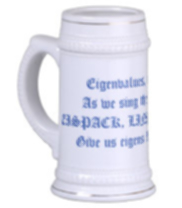
\includegraphics[width=0.3\textwidth]{eigendrink}
  \end{center}
%\caption{A gull}
\vspace{-24pt}
\end{wrapfigure}
Wir
\marginnote{
\qrcode{
https://www.youtube.com/watch?v=23uk6N0ZNmY}
}
wissen bereits: Ein Punkt heisst \textbf{Fixpunkt} einer Abbildung $\ga$, wenn er mit seinem Bild zusammenfällt ($P' = P$ oder $\ga(P) = P$ oder $A\V{r_P} =\V{r_P}$). Weiter gilt:

\begin{cdef}
Eine Gerade $g$ heisst \textbf{Fixgerade} einer Abbildung $\ga$, wenn ihr Bild $g'$ mit $g$ zusammenfällt: $g=g'$.
\end{cdef}

\begin{bem}
Beachte, dass eine Fixgerade nicht aus lauter Fixpunkten bestehen muss.
\end{bem}

\begin{cdef}
Eine Gerade, die aus lauter Fixpunkten besteht, heisst \textbf{Fixpunktgerade}.
\end{cdef}

\begin{bem}
Jede Fixpunktgerade ist auch Fixgerade, aber nicht umgekehrt.
\end{bem}

\begin{bsp}
\ \\[-4ex]
\begin{itemize}
\item Ist $\ga$ die Streckung mit dem Zentrum $O$ und einem Faktor $k\neq1$, so ist jede Gerade durch $O$ Fixgerade, aber nicht Fixpunktgerade.
\item Ist $\ga$ die Spiegelung an einer Geraden $g$, so ist $g$ Fixpunktgerade, und die dazu senkrechten Geraden sind Fixgeraden.
\item Eine Drehung um den Ursprung mit dem Drehwinkel $\varphi$ ($\varphi\neq n\cdot180^\circ$) hat keine Fixgeraden.
\end{itemize}
\end{bsp}

Klar ist, dass jede Ursprungsaffinität sicher einen Fixpunkt hat, nämlich den Ursprung $O$. Damit stellen sich für das weitere Vorgehen im Zusammenhang mit Matrizen die zwei folgenden Fragen:

\begin{itemize}
\item Existieren ausser $O$ noch weitere Fixpunkte? Und falls ja, unter welcher Bedingung?
\item Besitzt eine Ursprungsaffinität vielleicht auch Fixgeraden, und wie werden diese bestimmt?
\end{itemize}

Die Behandlung der zweiten Frage wird auf den Begriff des \emph{Eigenvektors} führen, der nicht nur hier, sondern auch bei ganz anderen Fragestellungen von Bedeutung ist.

\subsection{Fixpunkte bei Ursprungsaffinitäten}

Ausgangspunkt ist die Ursprungsaffinität
$$\glsysa{a_{11}x+a_{12}y}{a_{21}x+a_{22}y}.$$

Ein Punkt $P =(x|y)$ ist genau dann Fixpunkt, wenn $P' =(x'|y') =(x|y)=P$, d.h. wenn:
\begin{align*}
x &= a_{11}x+a_{12}y\\
y &= a_{21}x+a_{22}y
\end{align*}

Dieses Gleichungssystem wird häufig folgendermassen geschrieben:
\begin{align*}
(a_{11}-1)x+a_{12}y & = 0\\
a_{21}x+(a_{22}-1)y & = 0
\end{align*}

Es handelt sich hier um ein homogenes lineares Gleichungssystem (die Konstanten fehlen, bzw. sind Null). Ein solches Gleichungssystem hat in jedem Fall die sogenannte triviale Läsung $x = y = 0$. Ob noch weitere (nicht triviale) Läsungen existieren, hängt nun von der Determinante des Systems ab; also von
$$
\det(A-E)=
\begin{vmatrix}
a_{11}-1 & a_{12}\\
a_{21} & a_{22}-1
\end{vmatrix}
= (a_{11}-1)(a_{22}-1)-a_{12}a_{21}
$$

Es werden die folgenden Fälle unterschieden:
\begin{description}
\item[$D\neq0$:] Das System besitzt wegen der Bijektivität der durch das homogene Gleichungssystem repräsentierten Matrix nur eine, nämlich die triviale Läsung $x = y = 0$; d.h. es gibt ausser dem Ursprung keine weiteren Fixpunkte.
\item[$D=0$:] Neben der trivialen Läsung existieren unendlich viele, zusätzliche Läsungen. Die beiden Gleichungen des homogenen Gleichungssystems sind linear abhängig (Vielfache voneinander) und liefern somit redundante Informationen. Was bleibt ist eine (lineare) Gleichung, die gerade die Menge der Fixpunkte beschreibt. In diesem Fall existiert also eine Fixpunktgerade.

Ein Spezialfall liegt dann vor, wenn das homogene Gleichungssystem lauter Nullen aufweist, es sich also bei der Abbildungsmatrix $A$ um die Einheitsmatrix $E$ handelt. In diesem Fall ist jeder Punkt der Ebene ein Fixpunkt ($\ga$ ist die Identitätabbildung).
\end{description}

\subsection{Fixpunkte bei Affinitäten}

Von besonderem Interesse scheint der Fall zu sein, wenn eine Affinität genau
eine Fixpunktgerade besitzt. Man definiert

\begin{cdef}
Eine Affinität $\ga$, die genau eine Fixpunktgerade $g$ besitzt, wird \textbf{axiale} oder \textbf{perspektive Affinität} genannt. Ihre Fixpunktgerade $g$ heisst \textbf{Affinitätsachse}.
\end{cdef}

\begin{ueb}
Sei $\ga$ die Spiegelung an der Ursprungsgeraden $g$ mit Neigungswinkel $30^\circ$. Weise rechnerisch nach (u.a. durch Berechnung der Determinante des homogenen Systems), dass die Ursprungsgerade Fixpunktgerade ist.
\end{ueb}

\begin{ueb}
Bestimme die Menge der Fixpunkte der Abbildung
$$\glsysa{3x+y}{\phantom{3}x-y}.$$
\end{ueb}

\begin{ueb}
Zeige, dass die Affinität
$$\glsysa{2x-2y}{3x-5y}$$
eine axiale ist. Gib die Gleichung der Fixpunktgeraden und drei verschiedene Fixpunkte an.
\end{ueb}

\begin{ueb}
Bestimme die Menge der Fixpunkte der Abbildung
$$\glsysa{3x+y-1}{\phantom{3}x-y+2}.$$
\end{ueb}

\begin{ueb}
Die Punkte $P=(-1|5)$ und $Q=(3|1)$ sind Fixpunkte einer affinen Abbildung $\ga$. Zeige, dass dann die Gerade durch diese Punkte Affinitätsachse von $\ga$ sein muss.
Welche Konsequenzen kannst du jetzt allgemein daraus ziehen?
\end{ueb}

\begin{ueb}
Warum kann eine Affinität
$$\ga:\mR^2\longrightarrow\mR^2$$
nur eine Fixpunktgerade haben? Wie siehts im $\mR^3$ aus?
\end{ueb}

\begin{ueb}
Zeige, dass im $\mR^2$ folgendes gilt: Hat die Abbildung $\ga$ zwei verschiedene Fixpunktgeraden, so handelt es sich bei $\ga$ um die Identität.
\end{ueb}

\section{Fixgeraden bei Ursprungsaffinitäten}
Ausgangspunkt sei die Ursprungsaffinität $\ga$, die durch die folgende Matrixschreibweise gegeben ist:
$$\V{r'}=A\cdot\vr$$.

\begin{bem}
Bei der Bestimmung der Fixgeraden beschränken wir uns vorerst auf Ursprungsgeraden. (Man kann zeigen, dass gar keine anderen Geraden als Fixgeraden in Frage kommen, ausser wenn $\ga$ die Identität oder eine axiale Ursprungsaffinität darstellt.)
\end{bem}

Ist
\marginnote{
\qrcode{
https://www.youtube.com/watch?v=RcQY8_7eHuI}
}
jetzt $g$ eine Fixgerade, die durch den Ursprung verläuft, so muss jeder Geradenpunkt $P =(x|y)$ wieder auf einen Geradenpunkt $P'=(x'|y')$ abgebildet werden. Das bedeutet, dass der Ortsvektor $\V{r'}$ von $P'$ ein Vielfaches des Ortsvektors $\vr$ von $P$ sein muss. Es gibt also ein $\gl\in\mR$ so, dass:
$$\V{r'}=\gl\cdot\V{r}\q\text{oder}\q A\cdot\vr=\gl\cdot\vr.$$
Umgeformt wie im vorhergehenden Kapitel ergibt sich
\begin{align*}
(a_{11}-\gl)x+a_{12}y &= 0\\
a_{21}x+(a_{22}-\gl)y &= 0
\end{align*}

\begin{cdef}
Existiert ein Vektor
$$\vr=\pv{x}{y}\neq\V{0},$$
der obiges Gleichungssystem erfüllt, so heisst er \textbf{Eigenvektor} der Matrix $A$. Das zugehärige $\gl$ heisst \textbf{Eigenwert}.
\end{cdef}

\begin{bem}
Der Eigenvektor ist ein Richtungsvektor der Fixgeraden. Seine Länge spielt
dabei keine Rolle. Sie alle besitzen immer denselben Eigenwert $\gl$.
\end{bem}

Um die Eigenvektoren und Eigenwerte zu bestimmen, ist die Determinante des homogenen Systems von Wichtigkeit:
\begin{description}
\item[$\det(A-\gl E)\neq0$:] Das homogene System besitzt nur die triviale Läsung $x=y=0$; d.h. die Abbildungsmatrix besitzt keine Fixgerade.
\item[$\det(A-\gl E)=0$:] Die zugehärige Gleichung
$$\gl^2-(a_{11}+a_{22})\gl+\det(A)=0$$
heisst \textbf{charakteristische Gleichung} der Matrix $A$ und bestimmt ob, und falls ja, wie viele Fixgeraden die Abbildung $\ga$ besitzt.
\end{description}

\begin{bsp}
Bestimme die Eigenwerte, Eigenvektoren und Fixgeraden der Abbildung $\ga$, die durch die Matrix
$$A=\mat{1}{5}{2}{4}$$
und der Abbildung $\gb$, die durch die Matrix
$$B=\mat{3}{-1}{1}{1}$$
gegeben ist. Zeichne jeweils die Fixgeraden in die beiden Koordinatensysteme ein.
\begin{center}
\definecolor{cqcqcq}{rgb}{0.75,0.75,0.75}
\scalebox{1.1}{
\begin{tikzpicture}[line cap=round,line join=round,>=triangle 45,x=0.5cm,y=0.5cm]
\draw [color=cqcqcq,dash pattern=on 1pt off 1pt, xstep=0.5cm,ystep=0.5cm] (-5.5,-3.5) grid (6.5,5.5);
\draw[->,color=black] (-5.5,0) -- (6.5,0);
\foreach \x in {-4,-2,2,4,6}
\draw[shift={(\x,0)},color=black] (0pt,2pt) -- (0pt,-2pt) node[below] {\footnotesize $\x$};
\draw[color=black] (6.15,0.08) node [anchor=south west] {$x$};
\draw[->,color=black] (0,-3.5) -- (0,5.5);
\foreach \y in {-3,-2,-1,1,2,3,4,5}
\draw[shift={(0,\y)},color=black] (2pt,0pt) -- (-2pt,0pt) node[left] {\footnotesize $\y$};
\draw[color=black] (0.1,5.12) node [anchor=west] {$y$};
\draw[color=black] (0pt,-10pt) node[right] {\footnotesize $0$};
\clip(-5.5,-3.5) rectangle (6.5,5.5);
\end{tikzpicture}
}
\definecolor{cqcqcq}{rgb}{0.75,0.75,0.75}
\scalebox{1.1}{
\begin{tikzpicture}[line cap=round,line join=round,>=triangle 45,x=0.5cm,y=0.5cm]
\draw [color=cqcqcq,dash pattern=on 1pt off 1pt, xstep=0.5cm,ystep=0.5cm] (-5.5,-3.5) grid (6.5,5.5);
\draw[->,color=black] (-5.5,0) -- (6.5,0);
\foreach \x in {-4,-2,2,4,6}
\draw[shift={(\x,0)},color=black] (0pt,2pt) -- (0pt,-2pt) node[below] {\footnotesize $\x$};
\draw[color=black] (6.15,0.08) node [anchor=south west] {$x$};
\draw[->,color=black] (0,-3.5) -- (0,5.5);
\foreach \y in {-3,-2,-1,1,2,3,4,5}
\draw[shift={(0,\y)},color=black] (2pt,0pt) -- (-2pt,0pt) node[left] {\footnotesize $\y$};
\draw[color=black] (0.1,5.12) node [anchor=west] {$y$};
\draw[color=black] (0pt,-10pt) node[right] {\footnotesize $0$};
\clip(-5.5,-3.5) rectangle (6.5,5.5);
\end{tikzpicture}
}
\end{center}
\end{bsp}

\begin{ueb}
\ \\[-4ex]
\begin{enumeratea}
\item Wie viele verschiedene Eigenwerte kann eine Matrix haben?
\item Vermute einen Zusammenhang zwischen der Anzahl Eigenwerte und der Anzahl Fixgeraden.
\item Wie sieht es bei einer Streckung aus?
\end{enumeratea}
\end{ueb}

\subsection{Berechnungsbeispiele}

Eine Matrix $A$ kann also genau zwei, genau einen oder keinen Eigenwert haben. Zudem haben einem die †bungen der vorherigen Seite vor Augen geführt, dass aufgrund der Anzahl Eigenwerte nicht zwangsläufig auf die Anzahl Fixgeraden geschlossen werden kann. Im Folgenden sollen die drei Fälle noch etwas genauer anhand von Beispielen analysiert werden.

\begin{description}
\item[keine Eigenwerte] In diesem Fall besitzt die Ursprungsaffinität auch keine Fixgerade. Warum?
\begin{bsp}
Drehung um $O$ um den Winkel $\varphi\neq k\cdot180\circ$ mit $k\in\mZ$.
\end{bsp}
\item[genau ein Eigenwert] Wir haben gesehen, dass es zu einem Eigenwert durchaus auch mehrere Fixgeraden geben kann; genauer, unendlich viele. Dieser Fall kann aber nur dann eintreten, wenn die Matrix
$$\mat{a_{11}-\gl}{a_{12}}{a_{21}}{a_{22}-\gl}$$
die Nullmatrix ist (nur dann kännen $x$ und $y$ frei gewählt werden). Das bedeutet aber, dass in der Hauptdiagonalen überall $\gl$ stehen muss ($a_{11}=a_{22}=\gl$) und in der Nebendiagonalen lauter Nullen ($a_{12}=a_{21}=0$). Bei dieser Abbildung muss es sich also gerade um eine Streckung handeln.
In allen anderen Fällen (mit genau einem Eigenwert), hat man es mit einer Fixgeraden durch den Ursprung zu tun.
\begin{bsp}
Besitzt die Scherung
$$A\mat{1}{3}{0}{1}$$
wirklich nur eine Fixgerade?
\end{bsp}
\item[genau zwei Eigenwerte] In diesem Fall besitzt die Ursprungsaffinität zwei verschiedene, durch den Ursprung verlaufende Fixgeraden.
\begin{bsp}
Untersuche die Abbildung $\ga$ mit der Matrix
$$A=\mat{0}{1}{2}{-1}$$
auf Fixgeraden und zeichne sie ins unten stehende Koordinatensystem
\begin{center}
\definecolor{cqcqcq}{rgb}{0.75,0.75,0.75}
\scalebox{1.4}{
\begin{tikzpicture}[line cap=round,line join=round,>=triangle 45,x=0.5cm,y=0.5cm]
\draw [color=cqcqcq,dash pattern=on 1pt off 1pt, xstep=0.5cm,ystep=0.5cm] (-5.5,-3.5) grid (6.5,5.5);
\draw[->,color=black] (-5.5,0) -- (6.5,0);
\foreach \x in {-4,-2,2,4,6}
\draw[shift={(\x,0)},color=black] (0pt,2pt) -- (0pt,-2pt) node[below] {\footnotesize $\x$};
\draw[color=black] (6.15,0.08) node [anchor=south west] {$x$};
\draw[->,color=black] (0,-3.5) -- (0,5.5);
\foreach \y in {-3,-2,-1,1,2,3,4,5}
\draw[shift={(0,\y)},color=black] (2pt,0pt) -- (-2pt,0pt) node[left] {\footnotesize $\y$};
\draw[color=black] (0.1,5.12) node [anchor=west] {$y$};
\draw[color=black] (0pt,-10pt) node[right] {\footnotesize $0$};
\clip(-5.5,-3.5) rectangle (6.5,5.5);
\end{tikzpicture}
}
\end{center}
\end{bsp}

\end{description}

\begin{ueb}
\ \\[-4ex]
\begin{enumeratea}
\item Gibt es zu obiger Abbildung weitere Fixgeraden (die eventuell nicht durch den Ursprung verlaufen)? Skizziere.
\item Gegeben sei eine Matrix $A$, die zwei Eigenwerte $\gl\neq1\neq\gm$ besitzt. Es existieren also auch zwei verschiedene Fixgeraden, die durch den Ursprung verlaufen. Kann $A$ noch weitere Fixgeraden haben, die nicht durch den Ursprung verlaufen?
\end{enumeratea}
\end{ueb}

\subsection{Überblick}
Eine Ursprungsaffinität kann genau zwei verschiedene, genau einen oder keinen Eigenwert besitzen.
\begin{itemize}
\item Besitzt die Ursprungsaffinität zwei verschiedene Eigenwerte ungleich $1$, so existieren zwei verschiedene Ursprungsgeraden, die Fixgeraden sind.
\begin{itemize}
\item Hat einer der beiden Eigenwerte den Wert $1$, so wird die entsprechende Fixgerade $g_1$ zur Fixpunktgeraden und die Abbildung damit zu einer axialen oder perspektiven Ursprungsaffinität. Die Fixpunktgerade wird dann als \textbf{Affinitätsachse} bezeichnet. In diesem Fall gibt es weitere, unendlich viele Fixgeraden. Sie liegen parallel zur anderen Fixgeraden $g_2$.
\item Sind die Eigenwerte von $1$ verschieden, so existieren nur die beiden durch den Ursprung verlaufenden Fixpgeraden.
\end{itemize}
\item Besitzt die Ursprungsaffinität genau einen Eigenwert, so verläuft im Allgemeinen eine Fixgerade $g_1$ durch den Ursprung, ausser es handelt sich um eine Streckung am Ursprung; dann ist jede Ursprungsgerade Fixgerade.

Hat der Eigenwert den Wert $1$, so existieren noch weitere Fixgeraden, die alle parallel zur Fixgeraden $g_1$ verlaufen (vgl. Scherung).
\item Besitzt die Ursprungsaffinität keinen Eigenwert, so existieren auch keine Fixgeraden.
\end{itemize}

\begin{ueb}
Bestimme rechnerisch die Eigenwerte, Eigenvektoren und alle Fixgeraden der
\begin{enumeratea}
\item Spiegelung an einer Ursprungsgeraden mit dem Neigungswinkel $\varphi$,
\item Abbidlung $\gb$
$$\pv{x'}{y'}=\mat{-1}{-4}{6}{10}\pv{x}{y}$$
\item Abbidlung $\gg$
$$\pv{x'}{y'}=\mat{5}{0}{-3}{1}\pv{x}{y}$$
\item Abbidlung $\gd$
$$\pv{x'}{y'}=\mat{5}{1}{-1}{3}\pv{x}{y}$$
\end{enumeratea}
\end{ueb}

\begin{ueb}
Gegeben sei die Matrix
$$A=\mat{2}{-1}{p}{3}.$$
\begin{enumeratea}
\item Für welche $p$ hat die durch $A$ repräsentierte Abbildung zwei Fixgeraden, eine bzw. keine Fixgerade durch den Ursprung.
\item Wie muss $p$ gewählt werden, damit die eine Fixgerade die Gerade
$$g:y=\frac{2}{5}$$
ist?
\item Wie muss $p$ gewählt werden, damit $\ga$
\begin{enumeratei}
\item flächentreu und orientierungserhaltend
\item flächentreu und gegensinnig ist?
\end{enumeratei}
Wie sehen die entsprechenden Fixgeraden aus?
\end{enumeratea}
\end{ueb}

\subsection{Diagonalisieren}

\begin{cdef}
Eine
\marginnote{
\qrcode{
https://www.youtube.com/watch?v=FHEa4M5i8ck}
}
\textbf{Diagonalmatrix} ist eine Matrix, in der nur in der Hauptdiagonalen Werte stehen, die verschieden von Null sind. An allen anderen Stellen stehen lauter Nullen.
\end{cdef}

Besitzt die Matrix $A$ einer Ursprungsaffinität $\ga$ die verschiedenen Eigenwerte $\gl_1\neq\gl_2$ und damit auch zwei linear unabhängige
\footnote{Man kann zeigen, dass zu zwei verschiedenen Eigenwerten immer auch zwei linear unabhängige Eigenvektoren gehären.}
Eigenvektoren $\V{v_1}$ und $\V{v_2}$, so werden alle Punkte auf der Fixgeraden $g_1$ bzw. $g_2$ mit dem entsprechenden Faktor $\gl_1$ bzw. $\gl_2$ zentrisch vom Ursprung aus gestreckt. Damit ist die Ursprungsaffinität eindeutig bestimmt. Wäre $\set{\V{v_1},\V{v_2}}$ die
Basis unseres Koordinatensystems, so hätte die Matrix $A$ die Diagonalgestalt
$$\mat{\gl_1}{0}{0}{\gl_2}$$
und die Abbildung damit einfach zu verstehen. Leider sind sie es aber in der Regel nicht.

Dennoch, mit Hilfe eines Basiswechsels kann diese interpretationsfreundliche Situation geschaffen werden. Die Matrix $A$ der Ursprungsaffinität $\ga$ kann nämlich durch †berführen der Eigenvektoren $\V{v_1}, \V{v_2}$ in die Standardbasis $\ex, \ey$ (Matrix $X^{-1}$), anschliessendem Anwenden der Diagonalmatrix
$$D=\mat{\gl_1}{0}{0}{\gl_2}$$
und schliesslich Rücktransformation der
Standardbasis in die Eigenvektoren (Matrix $X$) ausgedrückt werden:
$$A=X\cdot D\cdot X^{-1}.$$
Die Spaltenvektoren des Basiswechsels $X$ entsprechen dabei gerade den Eigenvektoren $\V{v_1}, \V{v_2}$ Durch Linksmultiplikation mit $X^{-1}$ und Rechtsmultiplikation mit $X$ folgt daraus der folgende

\begin{satz}
Besitzt die Matrix $A$ zwei verschiedene Eigenwerte mit den Eigenvektoren $\V{v_1}, \V{v_2}$, so lässt sie sich durch die Matrix $X=(\V{v_1}, \V{v_2})$ diagonalisieren:
$$D=X^{-1}\cdot A\cdot X.$$
\end{satz}

Man sagt, dass $A$ durch $X$ \textbf{diagonalisiert} wird.

\begin{ueb}
Diagonalisieren Sie die Matrix
$$A=\mat{1}{2}{3}{2}.$$
\end{ueb}

\subsection{Potenzieren von Matrizen in Anwendungen}

\subsubsection{Verkehrszählung}

\begin{bsp}
Über Verkehrszählungen wurde ermittelt, dass $80\%$ der Pendler, die mit äffentlichen Verkehrsmitteln zur Arbeit fahren, auch im nächsten Jahr äffentliche Verkehrsmittel benützen wollen. $20\%$ bekunden allerdings aufs Auto umzusteigen. Von den Autofahren wollen auch im nächsten Jahr $60\%$ dem Auto treu bleiben, dagegen wollen $40\%$ auf äffentliche Verkehrsmittel wechseln. Ist $a_n$ die Zahl der Autofahrer im Jahr $n$, und steht $o_n$, für die Nutzerzahl des äffentlichen Nahverkehrs, dann kann dieses Verhalten als Matrixmultiplikation
$$\pv{a_{n+1}}{o_{n+1}}=\mat{0.6}{0.2}{0.4}{0.8}\cdot\pv{a_n}{o_n}$$
dargestellt werden.

Verkehrsplaner interessieren sich dabei für die Prognosen des Individual- und äffentlichen Verkehrs der nächsten Jahre; zum Beispiel, wie das Verkehrsverhalten in 10 Jahren aussehen wird. Also
$$
\pv{a_{10}}{o_{10}}=\mat{0.6}{0.2}{0.4}{0.8}\cdot\pv{a_9}{o_9}=\mat{0.6}{0.2}{0.4}{0.8}^2\cdot\pv{a_8}{o_8}=\dots=\mat{0.6}{0.2}{0.4}{0.8}^{10}\cdot\pv{a_0}{o_0}
$$
Es stellt sich also die Frage, wie Matrizen effizient potenziert werden kännen. Des weiteren interessiert vielleicht auch die Frage, ob es einen stationären Zustand gibt, also einen Zustand, bei dem sich über ein Jahr (und damit immer) keine zahlenmässigen Verschiebungen mehr ergeben. Das würde dem Fixpunkt der Abbildung entsprechen.
\end{bsp}

\subsubsection{Fibonacci-Zahlen und goldener Schnitt}

\begin{bsp}
Fibonacci-Zahlen sind bekanntlich durch die Rekursion
$$a_k=a_{k-1}+a_{k-2}$$
mit $a_1=a_2=1$ definiert.
Es stellt sich die Frage, wie das explizite Bildungsgesetz aussehen kännte.

Das rekursive Bildungsgesetz der Fibonacci-Folge kann auch mit Hilfe einer Matrix (etwas umständlich) angegeben werden:
$$\pv{a_k}{a_{k-1}}=\mat{1}{1}{1}{0}\cdot\pv{a_{k-1}}{a_{k-2}}.$$
\end{bsp}

\begin{ueb}
Wie
\marginnote{
\qrcode{
https://youtu.be/B8STr0FCW1E}
}
sieht das explizite Gesetz aus?
\end{ueb}

\begin{ueb}
Sind die folgenden Matrizen diagonalisierbar? Wenn ja diagonalisiere sie.
$$A=\mat{2}{0}{1}{2}, B=\mat{2}{-3}{1}{-1}, C=\mat{1}{0}{6}{-1}$$
\end{ueb}

\begin{ueb}
Berechne die 20. Potenz der Matrix
$$A=\mat{2}{2}{-1}{-2}.$$
\end{ueb}

\begin{ueb}
Es seien $A,B\in\text{Mat}(2\times2)$ invertierbar.
\begin{enumeratea}
\item Zeige, dass $(A\cdot B)^{-1}=B^{-1}\cdot A^{-1}.$
\item $A$ werde durch $X$ diagonalisiert. Zeige, dass auch $A^{-1}$ durch $X$ diagonalisiert wird.
\end{enumeratea}
\end{ueb}

\begin{cdef}
Eine Matrix $A$ heisst \textbf{symmetrisch}, wenn $a_{12}=a_{21}.$
\end{cdef}

\begin{ueb}
\ \\[-4ex]
\begin{enumeratea}
\item Zeige für die symmetrische Matrix
$$A=\mat{1}{2}{2}{-2},$$
dass ihre Eigenvektoren senkrecht aufeinander stehen.
\item Zeige für die symmetrische Matrix
$$B=\mat{1}{1}{1}{5},$$
dass ihre Eigenvektoren senkrecht aufeinander stehen.
\item Beweise obige Behauptung allgemein.
\item Zeige die Umkehrung: Stehen zwei Eigenvektoren einer Matrix $A$ senkrecht aufeinander, so ist die Matrix $A$ symmetrisch.
\end{enumeratea}
\end{ueb}

\begin{ueb}
Zeige, dass die rekursiv definierte Folge
$$a_k = 3a_{k-1} - 2a_{k-2}$$
mit $a_1 = 0$ und $a_2 = 1$ das explizite Bildungsgesetz $a_k = 2^{k-1} -1$ hat. (Kann auch mit vollständiger Induktion bewiesen werden.)
\end{ueb}

\begin{ueb}
Bestimme das explizite Bildungsgesetz der Folge
$$a_k = 3a_{k-1} + 4a_{k-2}$$
mit den Startwerten $a_1 =0$ und $a_2 =1$ bzw. $a_1 =-1$ und $a_2 =1$.
\end{ueb}

\begin{ueb}
Versuche --- falls mäglich --- eine allgemeine, explizite Formel für die rekursiv definierten Folgen der Art $$a_k = p \cdot a_{k-1} + q \cdot a_{k-2}$$
herzuleiten.
\end{ueb}

\subsection{Diagonalisieren von \glqq nicht-diagonalisierbaren\grqq\ Matrizen}

\begin{cdef}
Eine \textbf{obere} bzw. \textbf{untere Dreiecksmatrix} ist eine Matrix, deren Hauptdiagonalenelemente alle verschieden von Null sind ($a_{ii}\neq0$) und alle oberen Elemente $a_{ij} = 0$ für $i < j$ oder alle unteren Elemente $a_{ij} = 0$ für $i > j$.
\end{cdef}

\begin{bsp}
Die Matrix
$$A=
\begin{pmatrix}
1&3&0\\
0&2&2\\
0&0&-1
\end{pmatrix}$$
ist eine obere Dreiecksmatrix,
$$B=\mat{1}{0}{3}{1}$$
eine untere Dreiecksmatrix.
\end{bsp}

\begin{satz}
Die $n$-te Potenz einer (oberen/unteren) $2 \times 2$-Dreiecksmatrix $A$ ist wieder eine
(obere/untere) Dreiecksmatrix und berechnet sich durch
$$A^n=\mat{a_{11}}{a_{12}}{0}{a_{22}}^n=\mat{a_{11}^n}{b}{0}{a_{22}^n}$$
mit $b=a_{12}(a_{11}^{n-1}+a_{11}^{n-2}a_{22}+a_{11}^{n-3}a_{22}^2+\dots+a_{22}^{n-1}).$
\end{satz}

\begin{ueb}
Berechne
$$A=\mat{-1}{1}{0}{2}^5.$$
\end{ueb}

\begin{satz}
Das charakteristische Polynom einer $2 \times 2$-Matrix besitze eine (doppelte) Nullstelle, also einen einzigen Eigenwert. Dann existiert eine reguläre Matrix $X$ so, dass $X^{-1}\cdot A\cdot X$ eine (obere) Dreiecksmatrix ist, in deren Hauptdiagonale zweimal der Eigenwert steht.
\end{satz}

\begin{ueb}
Diagonalisiere die Matrix
$$A=\mat{1}{-1}{1}{3}$$
so weit als mäglich, d.h. bringe sie in Dreiecksgestalt.
\end{ueb}

\begin{ueb}
Bestimme das explizite Bildungsgesetz der rekursiv definierten Folgen
\begin{enumeratea}
\item $a_k=2a_{k-1}-a_{k-2}$ mit $a_1=0$ und $a_2=1$ bzw. $a_1=1$ und $a_2=4$,
\item $a_k=4a_{k-1}-a_{k-2}$ mit $a_1=0$ und $a_2=1$.
\end{enumeratea}
\end{ueb}

\begin{bem}
Besitzt eine Matrix keinen Eigenwert, so kann die Matrix natürlich nicht in Dreiecks- und schon gar nicht in Diagonalgestalt gebracht werden. Es gibt dann also keine Basis, entlang der \glqq gestreckt\grqq\ wird.

Es stellt sich heraus, dass es sich bei solch gearteten Matrizen um Abbildungen handelt, die unter anderem eine Drehung beinhalten. Eine abschliessende Betrachtung folgt.
\end{bem}

\newpage

\appendix

\section{Ausblick auf quadratische Matrizen höherer Ordnung}

Bis jetzt haben wir ausschliesslich affine Abbildungen des $\mR^2$ betrachtet. Natürlich kann die entwickelte Theorie auch auf Räume häherer Dimension übertragen werden. Vieles bleibt sich dabei gleich oder zumindest ähnlich. Im folgenden werden wir uns kurz mit $3 \times 3$-Matrizen auseinandersetzen:
$$\begin{pmatrix}
a_{11}&a_{12}&a_{13}\\
a_{21}&a_{22}&a_{23}\\
a_{31}&a_{32}&a_{33}\\
\end{pmatrix}$$
Die Determinante berechnet sich durch
\begin{align*}
\det(A)=&a_{11}a_{22}a_{33}+a_{12}a_{23}a_{31}+a_{13}a_{21}a_{32}\\
&-a_{13}a_{22}a_{31}-a_{12}a_{21}a_{31}-a_{11}a_{23}a_{32}
\end{align*}
und besitzt folgende Eigenschaften:

\begin{itemize}
\item $\det(A)=0\Leftrightarrow$ Es gibt einen von $\V{0}$ verschiedenen Vektor, der durch $A$ auf $\V{0}$ abgebildet wird.
\item $\det(A)=0\Leftrightarrow$ $A$ besitzt keine inverse Matrix.
\item $\det(A)=0\Leftrightarrow$ Die Zeilen- (und Spaltenvektoren) sind linear abhängig.
\end{itemize}

\begin{bem}
Der Eigenraum zu einem Eigenwert im $\mR^2$ war eindimensional (ausser bei einer Streckung). Im $\mR^3$ ist das ganze etwas vielfältiger. Existieren drei verschiedenen Eigenwerte, dann besitzen die Eigenräume zu den entsprechenden Eigenwerten jeweils die Dimension $1$. Existieren hingegen nur zwei verschiedene Eigenwerte (einer mit der Vielfachheit 1 und der andere mit der Vielfachheit 2), so kann derjenige mit der Vielfachheit 2 einen Eigenraum besitzen, der die Dimension 2 oder 1 hat. Der andere Eigenwert mit der Vielfachheit 1 besitzt hingegen zwangsläufig einen Eigenraum der Dimension 1. In diesem Zusammenhang wird von der mäglichen Diskrepanz von \textbf{algebraischer} versus \textbf{geometrischer Vielfachheit} gesprochen.
\end{bem}

\begin{ueb}
Diagonalisiere, wenn mäglich, die Matrizen
$$A=
\begin{pmatrix}
0&0&-2\\
1&2&1\\
1&0&3\\
\end{pmatrix}
\q\text{und}\q
B=
\begin{pmatrix}
1&0&0\\
1&2&0\\
-3&5&2\\
\end{pmatrix}$$
\end{ueb}

\begin{ueb}\label{ueb:mats}
Finde die Matrizen zu den folgenden Abbildungen
\begin{enumeratea}
\item Spiegelung am Nullpunkt.
\item Spiegelung an der $xy$-Ebene
\item Spiegelung an der $z$-Achse
\item Drehung um die $y$-Achse um $90^\circ$
\item Projektion auf die $xz$-Ebene.
\end{enumeratea}
\end{ueb}

\begin{ueb}
Berechne
\marginnote{
\qrcode{
https://www.youtube.com/watch?v=kZgzVFJgKxM}
}
die Determinanten der 5 Abbildungsmatrizen aus Übung \ref{ueb:mats}. Gibt es eine Gesetzmässigkeit, die das Vorzeichen der Determinante betrifft?
\end{ueb}

\begin{ueb}
Leite analog zum zweidimensionalen Fall das charakteristische Polynom zur Berechnung der Eigenwerte her.
\end{ueb}

\begin{ueb}
Seien
\begin{gather*}
A=
\begin{pmatrix}
0&1&0\\
-1&0&0\\
0&0&-1\\
\end{pmatrix}
, B=
\begin{pmatrix}
1&0&0\\
0&\frac{1}{\sqrt{2}}&\frac{1}{\sqrt{2}}\\
0&-\frac{1}{\sqrt{2}}&\frac{1}{\sqrt{2}}\\
\end{pmatrix},
\\[2ex]
C=
\begin{pmatrix}
0.6&0.8&0\\
0&0&1\\
0.8&-0.6&0\\
\end{pmatrix}
\end{gather*}

\begin{enumeratea}
\item Berechne die Eigenwerte und Eigenvektoren der drei Matrizen.
\item Welche der drei Matrizen sind orthogonal?
\item Welche geometrischen Abbildungen werden durch die Matrizen beschrieben?
\end{enumeratea}
\end{ueb}

\begin{ueb}
Sei $A$ die Spiegelung an der Geraden
$$g:\V{r}=t\pV{1}{1}{0}.$$
Finde die Matrix zur Abbildung $A$.
\end{ueb}

\begin{ueb}
Sei $A$ die Spiegelung an der Ebene
$$E:x-2y=0.$$
Finde die Matrix zur Abbildung $A$.
\end{ueb}

\begin{ueb}
Gegeben sei die Matrix
$$A=\frac{1}{17}
\begin{pmatrix}
1&-12&-12\\
-12&8&-9\\
-12&-9&8\\
\end{pmatrix}.$$

\begin{enumeratea}
\item Berechne die Eigenvektoren und Eigenwerte von $A$.
\item Zeige, dass es sich bei $A$ um eine Spiegelung handelt.
\item Gib die Koordinatengleichung der Spiegelungsebene an.
\item Bestimme $\det(A)$ fast ohne zu rechnen.
\end{enumeratea}
\end{ueb}

\cleardoublepage
\listoffigures
\listoftables
%\newpage
%\nocite{*}
%\bibliographystyle{plain}
%\bibliography{preamble/literaturgoogle}
\end{document} 